\documentclass[aspectratio=169,10pt]{beamer}

\usepackage[T1]{fontenc}
\usepackage[utf8]{inputenc}
\usepackage{microtype}
\usepackage{tgheros}
\usepackage[scaled=0.92]{inconsolata}
\renewcommand{\familydefault}{\sfdefault}
\usepackage{amsmath}
\usepackage{amssymb}
\usepackage{array}
\usepackage{booktabs}
\usepackage{graphicx}
\usepackage{multirow}
\usepackage{ragged2e}
\usepackage{tabularx}
\usepackage{tikz}
\usepackage[most]{tcolorbox}
\usepackage{pifont}
\usetikzlibrary{calc,positioning}

\definecolor{header}{HTML}{123B4A}
\definecolor{headerlight}{HTML}{D7E7EC}
\definecolor{accent}{HTML}{D98E32}
\definecolor{ink}{HTML}{222222}
\definecolor{muted}{HTML}{5A6770}
\definecolor{softgray}{HTML}{F3F5F6}
\definecolor{grayborder}{HTML}{D4D8DB}
\definecolor{goodgreen}{HTML}{2F7D4A}
\definecolor{warnred}{HTML}{9A3B2D}
\definecolor{bluehint}{HTML}{EDF4F8}

\newcommand{\decktextmargin}{0.62cm}
\newcommand{\frametitleleftinset}{\decktextmargin}

\setbeamersize{text margin left=\decktextmargin, text margin right=\decktextmargin}
\setbeamertemplate{navigation symbols}{}
\setbeamertemplate{headline}{}
\setbeamercolor{normal text}{fg=ink,bg=white}
\setbeamercolor{structure}{fg=header}
\setbeamercolor{frametitle}{fg=white,bg=header}
\setbeamercolor{page number in head/foot}{fg=muted,bg=white}
\setbeamercolor{block title}{fg=header,bg=softgray}
\setbeamercolor{block body}{fg=ink,bg=softgray}
\setbeamercolor{itemize item}{fg=accent}
\setbeamercolor{itemize subitem}{fg=accent}

\setbeamerfont{frametitle}{size=\normalsize,series=\bfseries}
\setbeamerfont{framesubtitle}{size=\small}
\setbeamerfont{title}{size=\Huge,series=\bfseries}
\setbeamerfont{subtitle}{size=\Large}
\setbeamerfont{page number in head/foot}{size=\footnotesize,series=\bfseries}
\setbeamerfont{block title}{size=\normalsize,series=\bfseries}
\setbeamerfont{block body}{size=\small}

\setbeamertemplate{itemize item}{\color{accent}\scriptsize\ding{110}}
\setbeamertemplate{itemize subitem}{\color{accent}\tiny\ding{118}}

\makeatletter
\newcommand{\pagenumberrightinset}{0.19cm}
\newcommand{\pagenumberbottominset}{0.20cm}
\newcommand{\deckpagenumbers}{{\ttfamily\usebeamerfont{page number in head/foot}\insertframenumber\kern0.1em/\kern0.1em\inserttotalframenumber}}
\newcommand{\fullbleedbox}[2]{%
  \makebox[0pt][l]{%
    \hspace*{-\decktextmargin}%
    \begin{beamercolorbox}[wd=\paperwidth,ht=#1,dp=0pt,#2]{frametitle}%
    \end{beamercolorbox}%
  }%
  \vspace*{#1}%
}
\newcommand{\deckpagenumberoverlay}{%
  \begin{tikzpicture}[remember picture,overlay]
    \node[
      anchor=south east,
      inner sep=0pt,
      text=muted,
      font=\ttfamily\footnotesize\bfseries
    ] at ([xshift=-\pagenumberrightinset,yshift=\pagenumberbottominset]current page.south east) {\deckpagenumbers};
  \end{tikzpicture}%
}
\let\plainpagenumberoverlay\deckpagenumberoverlay
\newcommand{\plainheaderband}[1]{%
  \begin{tikzpicture}[remember picture,overlay]
    \path[fill=header] (current page.north west) rectangle ([yshift=-#1]current page.north east);
  \end{tikzpicture}%
}
\setbeamertemplate{frametitle}{%
  \nointerlineskip%
  \begin{beamercolorbox}[wd=\paperwidth,ht=0.74cm,dp=0cm,sep=0pt]{frametitle}
    \vbox to 0.74cm{%
      \vfil
      \hspace*{\frametitleleftinset}%
      \parbox[t]{\textwidth}{%
        {\usebeamerfont{frametitle}\strut\insertframetitle\par}%
        \ifx\insertframesubtitle\@empty\else%
          {\usebeamerfont{framesubtitle}\color{headerlight}\insertframesubtitle\par}%
        \fi
      }%
      \vfil
    }%
  \end{beamercolorbox}%
}
\makeatother

\setbeamertemplate{footline}{%
  \leavevmode%
  \hbox{%
    \begin{beamercolorbox}[wd=\paperwidth,ht=2.25ex,dp=1.1ex]{page number in head/foot}%
    \end{beamercolorbox}%
  }%
  \deckpagenumberoverlay%
}

\renewcommand{\arraystretch}{1.18}
\newcolumntype{Y}{>{\RaggedRight\arraybackslash}X}
\newcolumntype{M}[1]{>{\centering\arraybackslash}m{#1}}

\newcommand{\code}[1]{\texttt{#1}}
\newcommand{\term}[1]{{\color{header}\textbf{#1}}}
\newcommand{\miniheading}[1]{\vspace{0.1cm}{\color{header}\bfseries #1}\par\vspace{0.06cm}}
\newcommand{\sourceline}[1]{}
\newcommand{\datasourceline}[1]{\vspace{0.14em}{\raggedright\scriptsize\color{muted}\textbf{Source:} #1\par}}
\newenvironment{callout}
  {\begin{tcolorbox}[colback=accent!7!white,colframe=accent,boxrule=0.5pt,arc=2mm,left=1.5mm,right=1.5mm,top=1mm,bottom=1mm]\small}
  {\end{tcolorbox}}

\tcbset{
  deckbox/.style={
    enhanced,
    boxrule=0.35pt,
    arc=2mm,
    colback=softgray,
    colframe=grayborder,
    left=1.5mm,
    right=1.5mm,
    top=1.1mm,
    bottom=1.1mm,
    boxsep=0.5mm
  }
}

\newenvironment{softbox}
  {\begin{tcolorbox}[deckbox]}
  {\end{tcolorbox}}

\newenvironment{pseudobox}
  {\begin{tcolorbox}[deckbox,colback=black!2!white]\ttfamily\small}
  {\end{tcolorbox}}

\newcommand{\MetricTile}[2]{%
  \begin{tcolorbox}[deckbox,colback=bluehint,title=\textbf{#1},fonttitle=\small\bfseries,coltitle=header]
  \small #2
  \end{tcolorbox}
}

\newcommand{\SectionDivider}[3]{%
  \begin{frame}[plain]
    \plainheaderband{0.78cm}
    \begin{tikzpicture}[remember picture,overlay]
      \node[
        anchor=center,
        align=center,
        text=ink,
        text width=0.86\paperwidth,
        font=\bfseries\fontsize{19}{23}\selectfont
      ] at ([yshift=0.18cm]current page.center) {#1};
      \fill[softgray] ([xshift=0.62cm,yshift=1.78cm]current page.south west) rectangle ([xshift=-0.62cm,yshift=1.94cm]current page.south east);
      \pgfmathsetmacro{\progressfraction}{(#2)/(#3)}
      \path let \p1 = ([xshift=0.62cm,yshift=1.78cm]current page.south west), \p2 = ([xshift=-0.62cm,yshift=1.94cm]current page.south east) in
        [fill=accent] (\p1) rectangle ({\x1 + \progressfraction*(\x2-\x1)}, \y2);
    \end{tikzpicture}
    \plainpagenumberoverlay
  \end{frame}
}

\newcommand{\AppendixDivider}[1]{%
  \begin{frame}[plain]
    \plainheaderband{0.78cm}
    \begin{tikzpicture}[remember picture,overlay]
      \node[
        anchor=center,
        align=center,
        text=ink,
        text width=0.88\paperwidth,
        font=\bfseries\fontsize{17}{21}\selectfont
      ] at ([yshift=0.18cm]current page.center) {#1};
      \fill[accent] ([xshift=0.62cm,yshift=1.78cm]current page.south west) rectangle ([xshift=-0.62cm,yshift=1.94cm]current page.south east);
    \end{tikzpicture}
    \plainpagenumberoverlay
  \end{frame}
}

\newcommand{\TitleFrame}[4]{%
  \begin{frame}[plain]
    \begin{tikzpicture}[remember picture,overlay]
      \path[fill=header] (current page.north west) rectangle ([yshift=-1.26cm]current page.north east);
      \path[fill=accent] ([yshift=-1.26cm]current page.north west) rectangle ([yshift=-1.38cm]current page.north east);
      \node[
        anchor=west,
        text=white,
        font=\bfseries\fontsize{19}{23}\selectfont
      ] at ([xshift=0.62cm,yshift=-0.70cm]current page.north west) {#1};
      \node[
        anchor=north west,
        align=left,
        text=header,
        text width=0.90\paperwidth,
        font=\bfseries\Large
      ] at ([xshift=0.62cm,yshift=-1.62cm]current page.north west) {#2};
    \end{tikzpicture}
    \vspace*{3.18cm}
    \begin{center}
      \begin{minipage}{0.88\textwidth}
        \begin{softbox}
          \small #3
        \end{softbox}
      \end{minipage}
    \end{center}
    \vspace{0.04cm}
    {\centering\small\color{muted}#4\par}
    \plainpagenumberoverlay
  \end{frame}
}

\graphicspath{{assets/}}

\begin{document}

\TitleFrame
  {PETSc Rewrite of Slope Stability}
  {From the legacy MATLAB workflow to the current PETSc runtime}
  {
    \begin{itemize}
      \item Translate the original MATLAB mental model into the current executable PETSc/Python path.
      \item Show where parallel ownership, PMG, unified runners, unified meshes, and unified visualisation changed the design.
    \end{itemize}
  }
  {Repository-local material only. Snapshot date: April 9, 2026.}

\begin{frame}{How I Structure This Talk}
\small
\begin{softbox}
\begin{itemize}
  \item I start from the legacy MATLAB scripts, because that is still the fastest shared mental model.
  \item I keep one concrete architecture anchor throughout: the checked-in 3D heterogeneous SSR benchmark that exercises the current \code{P4}/PMG path.
  \item Later I switch deliberately to the committed \code{P2} performance study, so architecture and runtime evidence never get mixed.
\end{itemize}
\end{softbox}
\end{frame}

\begin{frame}{Agenda}
\small
\begin{softbox}
\begin{enumerate}
  \item MATLAB baseline
  \item Prerequisites and getting running
  \item Structural redesign for parallelism
  \item Main new functionality
  \item Unified runners
  \item Unified visualisation
  \item Unified meshes
  \item Speed comparison
  \item Close and appendix
\end{enumerate}
\end{softbox}
\end{frame}

\begin{frame}{What I Use As Evidence}
\small
\begin{columns}[T,totalwidth=\textwidth]
\begin{column}{0.32\textwidth}
\MetricTile{Legacy MATLAB}{
\code{3D\_hetero\_SSR.m}\\
\code{+CONTINUATION/*}\\
\code{+NEWTON/*}\\
\code{+CONSTITUTIVE\_PROBLEM/*}\\
\code{+MESH/*}\\
\code{+VIZ/*}
}
\end{column}
\begin{column}{0.32\textwidth}
\MetricTile{PETSc Rewrite}{
\code{README.md}\\
\code{run\_config.py}\\
\code{run\_case\_from\_config.py}\\
\code{run\_3D\_hetero\_SSR\_capture.py}
}
\end{column}
\begin{column}{0.32\textwidth}
\MetricTile{Docs And Studies}{
\code{petsc\_matlab\_map}\\
\code{config\_scheme\_3d.md}\\
\code{config\_case\_matrix.md}\\
\code{performance\_comparison}
}
\end{column}
\end{columns}
\vspace{0.22cm}
\begin{softbox}
\miniheading{How I use them together}
The MATLAB tree gives the original mental model, the runtime code gives the current executable truth, and the docs package gives the shortest path through the mapping and the benchmark protocol. I use all three, but I do not substitute one for another.
\end{softbox}
\end{frame}

\SectionDivider{MATLAB Baseline}{1}{9}

\begin{frame}{The Legacy Execution Model Is Script-Centric}
\small
\begin{columns}[T,totalwidth=\textwidth]
\begin{column}{0.56\textwidth}
\begin{softbox}
\begin{itemize}
  \item One benchmark is usually one top-level script.
  \item \code{slope\_stability\_3D\_hetero\_SSR.m} declares the case, chooses the solver, launches continuation, and plots the results.
  \item The numerical kernels are modular, but orchestration remains case-local rather than registry-driven.
  \item The reader learns the workflow by reading the script from top to bottom.
\end{itemize}
\end{softbox}
\end{column}
\begin{column}{0.40\textwidth}
\begin{pseudobox}
quadrature\\
$\rightarrow$ local basis\\
$\rightarrow$ mesh load\\
$\rightarrow$ material expansion\\
$\rightarrow$ \code{K\_elast}, \code{B}, \code{f\_V}\\
$\rightarrow$ constitutive object\\
$\rightarrow$ SSR continuation\\
$\rightarrow$ MATLAB figures
\end{pseudobox}
\end{column}
\end{columns}
\sourceline{\code{slope\_stability\_matlab/slope\_stability\_3D\_hetero\_SSR.m}}
\end{frame}

\begin{frame}{MATLAB Package Map}
\small
\begin{tabularx}{\textwidth}{p{0.24\textwidth}p{0.33\textwidth}Y}
\toprule
\textbf{Package} & \textbf{Role} & \textbf{Typical content} \\
\midrule
\code{+ASSEMBLY} & FE preprocessing & Quadrature, local basis, elastic stiffness, volume forces, material expansion \\
\code{+CONTINUATION} & Outer branch tracking & Direct SSR, indirect SSR, LL, init phase, omega stepping \\
\code{+NEWTON} & Nonlinear solve core & Damped Newton, indirect SSR Newton, LL Newton \\
\code{+CONSTITUTIVE\_PROBLEM} & Stress and tangent model & Davis reduction, stress evaluation, tangent assembly, potential \\
\code{+LINEAR\_SOLVERS} & Linear solver factory & Direct, AGMG, ICHOL, HYPRE BoomerAMG, DFGMRES, collectors \\
\code{+MESH}, \code{+VIZ}, \code{+SEEPAGE} & Domain-specific helpers & Case loaders, plotting, seepage preprocessing and flow solve \\
\bottomrule
\end{tabularx}
\sourceline{\code{slope\_stability\_matlab/+ASSEMBLY}; \code{slope\_stability\_matlab/+CONTINUATION}; \code{slope\_stability\_matlab/+VIZ}}
\end{frame}

\begin{frame}{MATLAB Core Solver Loop}
\small
\begin{columns}[T,totalwidth=\textwidth]
\begin{column}{0.49\textwidth}
\begin{softbox}
\miniheading{Accepted-step lifecycle}
\begin{itemize}
  \item Continuation chooses the next \(\omega\) target.
  \item A secant-style predictor proposes \((U,\lambda)\).
  \item \code{NEWTON.newton\_ind\_SSR} solves the coupled equilibrium system.
  \item On success, history arrays grow and the deflation basis is updated.
  \item On failure, the step is shrunk and retried.
\end{itemize}
\end{softbox}
\end{column}
\begin{column}{0.49\textwidth}
\begin{softbox}
\miniheading{Main data objects}
\begin{itemize}
  \item \code{coord}, \code{elem}, \code{surf}, \code{Q}
  \item \(\,K_{\mathrm{elast}}, B, f_V\,\)
  \item Integration-point material fields: \(c_0, \phi, \psi, \gamma\)
  \item History outputs: \(\lambda\), \(\omega\), \(u_{\max}\), work counters
  \item Linear solver object copied into continuation calls
\end{itemize}
\end{softbox}
\end{column}
\end{columns}
\sourceline{\code{slope\_stability\_matlab/+CONTINUATION/SSR\_indirect\_continuation.m}; \code{slope\_stability\_matlab/+NEWTON/newton\_ind\_SSR.m}}
\end{frame}

\begin{frame}{The MATLAB Constitutive Object Is The Main Stateful Kernel Wrapper}
\small
\begin{columns}[T,totalwidth=\textwidth]
\begin{column}{0.57\textwidth}
\begin{softbox}
\begin{itemize}
  \item \code{CONSTITUTIVE\_PROBLEM.CONSTITUTIVE} stores the global strain-displacement matrix \(B\), quadrature weights, material fields, and runtime measurements.
  \item It performs Davis reduction for a given \(\lambda\), evaluates stress, evaluates the consistent tangent, and assembles residual and tangent objects.
  \item In other words, MATLAB centralises constitutive state in one handle object but feeds it with globally assembled FE operators.
\end{itemize}
\end{softbox}
\end{column}
\begin{column}{0.39\textwidth}
\begin{pseudobox}
reduction($\lambda$)\\
$\rightarrow$ stress(\(U\))\\
$\rightarrow$ stress+tangent(\(U\))\\
$\rightarrow$ build \(F\)\\
$\rightarrow$ build \(F, K_{\text{tangent}}\)\\
$\rightarrow$ return timings
\end{pseudobox}
\end{column}
\end{columns}
\sourceline{\code{slope\_stability\_matlab/+CONSTITUTIVE\_PROBLEM/CONSTITUTIVE.m}}
\end{frame}

\begin{frame}{Mesh Handling In MATLAB Is Closely Coupled To Element Degree}
\small
\begin{tabularx}{\textwidth}{p{0.28\textwidth}p{0.30\textwidth}Y}
\toprule
\textbf{MATLAB path} & \textbf{What it assumes} & \textbf{Consequence} \\
\midrule
\code{load\_mesh\_P2.m} & Quadratic tetrahedral HDF5 input & Benchmark meshes and FE degree are tied together \\
\code{load\_mesh\_gmsh\_waterlevels.m} & Case-specific Gmsh seepage conventions & Loader logic lives with the case family \\
\code{midpoints\_P2.m}, \code{midpoints\_P4.m} & Degree-specific node generation & Higher order support is added through dedicated utilities \\
\code{Q} mask from face labels & Boundary conditions embedded in the loader path & Free-DOF extraction depends on the loaded mesh convention \\
\bottomrule
\end{tabularx}
\vspace{0.18cm}
\begin{callout}
This is one of the biggest conceptual changes in the rewrite: the PETSc side moves toward \term{canonical mesh family storage} plus \term{solver-side degree selection}, instead of one file format per numerical path.
\end{callout}
\sourceline{\code{slope\_stability\_matlab/+MESH/load\_mesh\_P2.m}; \code{slope\_stability\_matlab/+MESH/load\_mesh\_gmsh\_waterlevels.m}}
\end{frame}

\begin{frame}{MATLAB Visualisation Still Lives Inside The Case Script}
\small
\begin{columns}[T,totalwidth=\textwidth]
\begin{column}{0.56\textwidth}
\begin{softbox}
\miniheading{What the MATLAB flow still does well}
\begin{itemize}
  \item The benchmark script can call \code{VIZ.*} immediately after the solve and inspect the same assembled state.
  \item That keeps the familiar 3D and slice figures close to the benchmark logic the original authors already know.
\end{itemize}
\end{softbox}
\begin{softbox}
\miniheading{What stays coupled}
\begin{tabularx}{\linewidth}{p{0.30\linewidth}Y}
\textbf{state} & live MATLAB workspace after the solve \\
\textbf{plots} & benchmark-local \code{VIZ.*} calls and figure setup \\
\textbf{reuse} & copy-and-adapt workflow between benchmark families \\
\end{tabularx}
\end{softbox}
\end{column}
\begin{column}{0.40\textwidth}
\begin{pseudobox}
solve benchmark\\
\(\rightarrow\) call \code{VIZ.*}\\
\(\rightarrow\) inspect figure state\\
\(\rightarrow\) export figure manually\\
\(\rightarrow\) repeat per case family
\end{pseudobox}
\vspace{0.18cm}
\begin{callout}
In the rewrite I keep the figure family as an outcome, but I stop depending on case-local plotting code and live interpreter state to rebuild it.
\end{callout}
\end{column}
\end{columns}
\end{frame}

\SectionDivider{Prerequisites And Getting Running}{2}{9}

\begin{frame}{Environment And Bootstrap}
\small
\begin{columns}[T,totalwidth=\textwidth]
\begin{column}{0.56\textwidth}
\begin{pseudobox}
\$ ./bootstrap.sh\\
\$ BOOTSTRAP\_MODE=wheel ./bootstrap.sh
\end{pseudobox}
\begin{softbox}
\begin{itemize}
  \item Default bootstrap creates \code{.venv}, builds PETSc with HYPRE under \code{.build}, installs \code{petsc4py}, and installs the project in editable mode.
  \item The wheel mode is lighter, but it may omit the full benchmark-capable PETSc/HYPRE stack.
  \item The repository is designed around a real local PETSc build, not just pure-Python smoke execution.
\end{itemize}
\end{softbox}
\end{column}
\begin{column}{0.40\textwidth}
\MetricTile{What the heavy first run buys you}{
\code{petsc4py}\\
HYPRE-enabled PETSc\\
editable install of \code{slope\_stability}\\
benchmark partitioning extras\\
notebook-ready environment
}
\end{column}
\end{columns}
\sourceline{\code{README.md}}
\end{frame}

\begin{frame}{Run One Case Or Run The Whole Benchmark Suite}
\small
\begin{columns}[T,totalwidth=\textwidth]
\begin{column}{0.53\textwidth}
\miniheading{Single case from a config}
\begin{pseudobox}
\$ ./.venv/bin/python -m\\
\ \ slope\_stability.cli.run\_case\_from\_config\\
\ \ benchmarks/run\_3D\_hetero\_SSR\_capture/case.toml\\
\ \ --out\_dir /tmp/ssr\_run
\end{pseudobox}
\miniheading{Canonical suite}
\begin{pseudobox}
\$ ./.venv/bin/python -m\\
\ \ slope\_stability.cli.run\_benchmark\_suite
\end{pseudobox}
\end{column}
\begin{column}{0.43\textwidth}
\begin{softbox}
\begin{itemize}
  \item A benchmark folder can also be run locally with its \code{run.sh}.
  \item The canonical MATLAB-parity subset is the set of folders whose \code{[benchmark].suite = true}.
  \item This unifies direct execution, suite execution, and notebook reuse around the same \code{case.toml}.
\end{itemize}
\end{softbox}
\end{column}
\end{columns}
\sourceline{\code{README.md}; \code{benchmarks/README.md}}
\end{frame}

\begin{frame}{Devcontainer And Standard Outputs}
\small
\begin{columns}[T,totalwidth=\textwidth]
\begin{column}{0.48\textwidth}
\begin{softbox}
\miniheading{Devcontainer}
\begin{itemize}
  \item The repository ships a prebuild-friendly \code{.devcontainer}.
  \item Slow setup can be absorbed into Codespaces prebuilds.
  \item Validation entry point: \code{bash .devcontainer/validate.sh --imports-only}
\end{itemize}
\end{softbox}
\end{column}
\begin{column}{0.48\textwidth}
\begin{softbox}
\miniheading{Outputs every config-driven run can write}
\begin{itemize}
  \item \code{exports/run\_debug.h5}
  \item \code{exports/continuation\_history.json}
  \item \code{exports/final\_solution.vtu}
  \item \code{exports/resolved\_config.toml}
\end{itemize}
\end{softbox}
\end{column}
\end{columns}
\vspace{0.18cm}
\begin{callout}
The rewrite standardises what MATLAB often kept as script-local variables or ad hoc figure state: the final mesh, the final fields, the continuation history, and the resolved runtime configuration.
\end{callout}
\sourceline{\code{README.md}; \code{docs/config\_case\_matrix.md}}
\end{frame}

\begin{frame}{Benchmark Folders Are The User-Facing Contract}
\small
\begin{tabularx}{\textwidth}{p{0.24\textwidth}p{0.19\textwidth}Y}
\toprule
\textbf{Item} & \textbf{Required?} & \textbf{Purpose} \\
\midrule
\code{case.toml} & yes & Runtime configuration and benchmark metadata \\
\code{run.sh} & yes & Local convenience entry point \\
\code{README.md} & yes & Human-facing explanation of the case \\
\code{[benchmark]} section & yes & Title, MATLAB script link, comparison kind, suite inclusion, MPI ranks \\
\code{[notebook]} section & optional but important & Controls the generated simulation and visualisation notebooks \\
\code{artifacts/simulation/*} & generated & Reusable outputs for notebooks and postprocessing \\
\bottomrule
\end{tabularx}
\sourceline{\code{benchmarks/README.md}; \code{benchmarks/generate\_benchmark\_notebooks.py}}
\end{frame}

\SectionDivider{Structural Redesign For Parallelism}{3}{9}

\begin{frame}{Responsibility Map: MATLAB Driver To PETSc Modules}
\small
\begin{tabularx}{\textwidth}{p{0.25\textwidth}p{0.26\textwidth}Y}
\toprule
\textbf{Role} & \textbf{MATLAB location} & \textbf{PETSc location} \\
\midrule
Case declaration & Top of the benchmark script & \code{case.toml} + \code{run\_config.py} \\
Runner dispatch & Implicit in the script name & \code{run\_case\_from\_config.py} \\
Mesh and material preprocessing & Script body + \code{+MESH}/\code{+ASSEMBLY} & \code{mesh/*} + \code{fem/*} + runner setup \\
Constitutive handle construction & \code{CONSTITUTIVE.m} & \code{problem.py:ConstitutiveOperator} \\
Continuation launch & \code{SSR\_indirect\_continuation.m} & \code{continuation/indirect.py} \\
Linear solver factory & \code{set\_linear\_solver.m} & \code{solver.py:SolverFactory} \\
\bottomrule
\end{tabularx}
\sourceline{\code{docs/petsc\_matlab\_map/chapters/mainline/01\_execution\_map.tex}}
\end{frame}

\begin{frame}{This Is The Architecture Anchor I Keep Coming Back To}
\small
\begin{softbox}
\miniheading{The benchmark I use as the walk-through case}
I use the checked-in 3D heterogeneous SSR default benchmark as the architecture anchor because it keeps the owned-row, overlap, \code{pmg\_shell}, and \code{P4} path in one place:
\begin{tabularx}{\linewidth}{@{}Y Y@{}}
\code{analysis = ssr} & \code{elem\_type = P4} \\
\code{node\_ordering = block\_metis} & \code{mpi\_distribute\_by\_nodes = true} \\
\code{constitutive\_mode = overlap} & \code{tangent\_kernel = rows} \\
\code{pc\_backend = pmg\_shell} & \\
\end{tabularx}
\end{softbox}
\vspace{0.16cm}
\begin{pseudobox}
load config $\rightarrow$ choose 3D SSR runner $\rightarrow$ load and reorder mesh\\
$\rightarrow$ build owned elastic rows $\rightarrow$ prepare owned tangent pattern\\
$\rightarrow$ create constitutive operator $\rightarrow$ build PETSc solver\\
$\rightarrow$ launch indirect SSR continuation
\end{pseudobox}
\vspace{0.10cm}
\begin{callout}
I use this case to explain the current architecture. The committed \code{P2} timings later answer a different question.
\end{callout}
\end{frame}

\begin{frame}{Config Load And Runner Dispatch}
\small
\begin{columns}[T,totalwidth=\textwidth]
\begin{column}{0.54\textwidth}
\begin{softbox}
\miniheading{Config side}
\begin{itemize}
  \item \code{core/run\_config.py} loads TOML, resolves relative paths, validates \code{elem\_type}, analysis kind, materials, and public section shapes.
  \item The config object preserves the same high-level blocks MATLAB already used: problem, continuation, Newton, linear solver, and outputs.
  \item Material rows can be provided explicitly or inherited from the mesh-family definition.
\end{itemize}
\end{softbox}
\end{column}
\begin{column}{0.42\textwidth}
\begin{pseudobox}
cfg = load\_run\_case\_config(...)\\
case = cfg.problem.case\\
runner, kwargs =\\
\ \ \_case\_runner\_kwargs(cfg)\\
result = runner(**kwargs)\\
write debug bundle\\
write history\\
write VTU
\end{pseudobox}
\end{column}
\end{columns}
\sourceline{\code{src/slope\_stability/core/run\_config.py}; \code{src/slope\_stability/cli/run\_case\_from\_config.py}}
\end{frame}

\begin{frame}{Assembly Policy And Node Ownership Are First-Class Decisions}
\small
\begin{columns}[T,totalwidth=\textwidth]
\begin{column}{0.50\textwidth}
\begin{softbox}
\miniheading{Policy inputs}
\begin{itemize}
  \item \code{solver\_type}
  \item \code{mpi\_distribute\_by\_nodes}
  \item \code{constitutive\_mode}
  \item \code{node\_ordering}
\end{itemize}
\miniheading{Default outcome}
\begin{itemize}
  \item owned tangent path enabled
  \item lightweight MPI elastic path enabled
  \item node numbering aligned to ownership through \code{block\_metis}
\end{itemize}
\end{softbox}
\end{column}
\begin{column}{0.46\textwidth}
\begin{callout}
\textbf{Why this matters}\\[0.12cm]
MATLAB kept one global sparse operator in one address space.\\[0.18cm]
The PETSc rewrite makes row ownership explicit early, because that ownership controls:
\begin{itemize}
  \item local element overlap
  \item constitutive work placement
  \item matrix assembly
  \item preconditioner construction
\end{itemize}
\end{callout}
\end{column}
\end{columns}
\sourceline{\code{src/slope\_stability/cli/assembly\_policy.py}; \code{docs/petsc\_matlab\_map/chapters/mainline/02\_mesh\_materials\_load.tex}}
\end{frame}

\begin{frame}{Owned Elastic Rows And A Fixed Tangent Pattern}
\small
\begin{columns}[T,totalwidth=\textwidth]
\begin{column}{0.48\textwidth}
\MetricTile{Prepared once}{
\begin{itemize}
  \item rank-owned node interval
  \item overlap elements for those rows
  \item local CSR matrix pattern
  \item elastic values on that pattern
  \item constrained diagonal positions
\end{itemize}
}
\end{column}
\begin{column}{0.48\textwidth}
\MetricTile{Refreshed every Newton step}{
\begin{itemize}
  \item constitutive state on overlap integration points
  \item internal force rows
  \item tangent values on the fixed CSR pattern
  \item regularised matrix blend \(K_r\)
\end{itemize}
}
\end{column}
\end{columns}
\vspace{0.18cm}
\begin{callout}
This is the deepest structural change relative to MATLAB: the rewrite no longer treats every Newton step as a fresh global sparse rebuild. The \term{structure} is prepared once; the \term{values} are refreshed in place.
\end{callout}
\sourceline{\code{src/slope\_stability/fem/distributed\_elastic.py}; \code{src/slope\_stability/fem/distributed\_tangent.py}}
\end{frame}

\begin{frame}{Overlap Constitutive Ownership And The Rows Kernel}
\small
\begin{columns}[T,totalwidth=\textwidth]
\begin{column}{0.49\textwidth}
\begin{softbox}
\miniheading{Overlap constitutive mode}
\begin{itemize}
  \item Each rank evaluates the constitutive model on the overlap integration points needed by its owned rows.
  \item The default path avoids a unique-owner recovery stage.
  \item The tangent kernel receives local overlap data directly.
\end{itemize}
\end{softbox}
\end{column}
\begin{column}{0.49\textwidth}
\begin{softbox}
\miniheading{Rows kernel}
\begin{itemize}
  \item The kernel walks the fixed owned CSR pattern row by row.
  \item Metadata such as \code{row\_slot\_ptr}, \code{slot\_elem}, \code{slot\_lrow}, and \code{slot\_pos} replace the old ``assemble element matrix, then scatter'' view.
  \item The bilinear form is unchanged; the dataflow is not.
\end{itemize}
\end{softbox}
\end{column}
\end{columns}
\sourceline{\code{docs/petsc\_matlab\_map/chapters/mainline/05\_tangent\_assembly.tex}; \code{src/slope\_stability/fem/distributed\_tangent.py}}
\end{frame}

\begin{frame}{What \code{pmg\_shell} Means On This Mainline}
\small
\begin{columns}[T,totalwidth=\textwidth]
\begin{column}{0.53\textwidth}
\begin{softbox}
\begin{itemize}
  \item The fine-grid operator is the reduced free-space regularized operator coming from the owned-row tangent path.
  \item The outer Krylov family is still the PETSc-wrapped MATLAB-style deflated FGMRES interface.
  \item The actual preconditioner is a custom shell V-cycle, not the built-in PETSc \code{PCMG} path.
  \item The hierarchy metadata enters through \code{pmg\_hierarchy} and stays aligned with the same reordered free-space numbering as the solve operator.
\end{itemize}
\end{softbox}
\end{column}
\begin{column}{0.43\textwidth}
\begin{tabularx}{\linewidth}{p{0.32\linewidth}Y}
\toprule
\textbf{MATLAB intuition} & one current sparse system plus one solver handle \\
\midrule
\textbf{PETSc mainline} & current reduced operator plus shell hierarchy plus chosen outer KSP \\
\bottomrule
\end{tabularx}
\vspace{0.16cm}
\begin{callout}
When I say ``parallel PMG'' in this repository today, this shell-preconditioned reduced solve is the path I mean.
\end{callout}
\end{column}
\end{columns}
\end{frame}

\begin{frame}{How The PMG Hierarchy Is Built And Rebuilt}
\small
\begin{columns}[T,totalwidth=\textwidth]
\begin{column}{0.50\textwidth}
\begin{pseudobox}
runner startup:\\
\ \ build reordered \code{pmg\_hierarchy}\\
\ \ default P4 chain: \(P1 \rightarrow P2 \rightarrow P4\)\\
\ \ store free-space levels + prolongations\\[0.08cm]
Newton step \(n\):\\
\ \ pass current reduced operator\\
\ \ validate level sizes + ownership\\
\ \ configure shell V-cycle on live matrix
\end{pseudobox}
\end{column}
\begin{column}{0.46\textwidth}
\begin{softbox}
\begin{itemize}
  \item The hierarchy geometry and transfer metadata are built once from the reordered mesh family, element order, and material rows.
  \item \code{\_ensure\_pmg\_state()} then turns those level-to-level transfers into PETSc matrices.
  \item The rebuild policy is still \code{every\_newton}: the shell preconditioner is reconfigured on the current operator each Newton step.
  \item So the multilevel layout is stable, while the fine-grid matrix and smoother state stay current.
\end{itemize}
\end{softbox}
\end{column}
\end{columns}
\end{frame}

\begin{frame}{How The Outer Krylov Solve Sits On Top Of PMG}
\small
\begin{columns}[T,totalwidth=\textwidth]
\begin{column}{0.48\textwidth}
\begin{pseudobox}
\(U,\lambda\) predictor\\
$\rightarrow$ refresh stress and tangent rows\\
$\rightarrow$ build reduced \(K_r\)\\
$\rightarrow$ outer deflated FGMRES sees \(A_f\)\\
$\rightarrow$ \code{pmg\_shell} applies V-cycle\\
$\rightarrow$ correction returns to Newton
\end{pseudobox}
\end{column}
\begin{column}{0.48\textwidth}
\begin{softbox}
\begin{itemize}
  \item \code{solver\_type} still selects the outer MATLAB-style deflated FGMRES wrapper.
  \item \code{pc\_backend = pmg\_shell} selects the shell V-cycle that lives inside each outer Krylov step.
  \item The \code{mg\_*} options then choose smoother behavior and the coarse-grid backend.
\end{itemize}
\end{softbox}
\vspace{0.12cm}
\begin{callout}
That is why I no longer read \code{solver\_type} in isolation. The real linear solve lives in the combination of the outer wrapper and the PMG-shell backend under it.
\end{callout}
\end{column}
\end{columns}
\end{frame}

\begin{frame}{What Changed Structurally To Enable Parallel Capabilities}
\small
\begin{columns}[T,totalwidth=\textwidth]
\begin{column}{0.24\textwidth}
\MetricTile{Case spec extracted}{
Problem definition moved out of the script body and into TOML plus mesh-family metadata.
}
\end{column}
\begin{column}{0.24\textwidth}
\MetricTile{Ownership explicit}{
Node ordering, owned rows, and overlap elements are selected before the nonlinear loop starts.
}
\end{column}
\begin{column}{0.24\textwidth}
\MetricTile{Assembly split}{
Matrix structure is prepared once, while values are refreshed in distributed kernels.
}
\end{column}
\begin{column}{0.24\textwidth}
\MetricTile{Solve stack decoupled}{
Outer Krylov logic, preconditioner backend, rebuild policy, and exports are independent surfaces.
}
\end{column}
\end{columns}
\vspace{0.16cm}
\begin{callout}
This is why the rewrite scales conceptually better than ``MATLAB script + MPI wrapper''. The parallelism is in the native architecture, not around it.
\end{callout}
\sourceline{\code{src/slope\_stability/cli/assembly\_policy.py}; \code{src/slope\_stability/fem/distributed\_tangent.py}; \code{src/slope\_stability/linear/solver.py}}
\end{frame}

\SectionDivider{Main New Functionality}{4}{9}

\begin{frame}{Shared Registry Across Benchmark Folders}
\small
\begin{columns}[T,totalwidth=\textwidth]
\begin{column}{0.32\textwidth}
\MetricTile{MATLAB-parity suite}{
5 canonical parity cases are listed in \code{benchmarks/README.md}, each with MATLAB and PETSc timing summaries.
}
\end{column}
\begin{column}{0.32\textwidth}
\MetricTile{Additional runnable cases}{
The registry also carries LL, 2D, 3D, seepage, and SIOPT cases that are not part of the parity suite.
}
\end{column}
\begin{column}{0.32\textwidth}
\MetricTile{Shared metadata}{
Each folder uses the same \code{[benchmark]} contract, the same config runner, and the same notebook generation flow.
}
\end{column}
\end{columns}
\vspace{0.18cm}
\begin{softbox}
Once the folder contract exists, the shared registry becomes the cross-case surface: it lets me select suites, compare parity cases, generate notebooks, and automate over many benchmarks without changing the execution model.
\end{softbox}
\sourceline{\code{benchmarks/README.md}}
\end{frame}

\begin{frame}{Richer Continuation And Solver Controls}
\small
\begin{tabularx}{\textwidth}{p{0.28\textwidth}p{0.28\textwidth}Y}
\toprule
\textbf{Interface} & \textbf{Examples in the rewrite} & \textbf{Why it matters} \\
\midrule
\code{[continuation]} & predictor, omega controller, warm-start mode, fine switch, step-length cap & Continuation behavior is no longer hidden inside one script variant \\
\code{[newton]} & stopping criterion, stopping tolerance, damping parameters & Stop conditions are explicit and comparable across studies \\
\code{[linear\_solver]} & backend, rebuild policy, Hypre/GAMG/BDDC options, recycle flag & Solver studies can be expressed in config instead of local script edits \\
\code{[execution]} & node ordering, ownership mode, tangent kernel & Parallel structure is public and reproducible \\
\bottomrule
\end{tabularx}
\sourceline{\code{src/slope\_stability/core/run\_config.py}; \code{docs/config\_scheme\_3d.md}}
\end{frame}

\begin{frame}{Structured Exports And Notebook Workflow}
\small
\begin{pseudobox}
run case from config\\
$\rightarrow$ save \code{run\_debug.h5}\\
$\rightarrow$ save \code{continuation\_history.json}\\
$\rightarrow$ save \code{final\_solution.vtu}\\
$\rightarrow$ save \code{resolved\_config.toml}\\
$\rightarrow$ reuse them in generated notebooks and external tools
\end{pseudobox}
\vspace{0.16cm}
\begin{columns}[T,totalwidth=\textwidth]
\begin{column}{0.49\textwidth}
\begin{softbox}
\miniheading{What this improves}
\begin{itemize}
  \item reproducibility
  \item postprocessing outside the solver process
  \item notebook regeneration without rerunning the case
  \item standard field names for PyVista and ParaView
\end{itemize}
\end{softbox}
\end{column}
\begin{column}{0.49\textwidth}
\begin{softbox}
\miniheading{MATLAB comparison}
\begin{itemize}
  \item MATLAB often kept these objects in workspace structs or figure state.
  \item The rewrite promotes them into stable file outputs.
  \item That is what enables the ``unified visualisation'' story later in the deck.
\end{itemize}
\end{softbox}
\end{column}
\end{columns}
\sourceline{\code{README.md}; \code{src/slope\_stability/export.py}; \code{benchmarks/prepare\_committed\_notebook\_artifacts.py}}
\end{frame}

\begin{frame}{The Rewrite Also Carries A P4 Export And 3D Display Path}
\small
\begin{columns}[T,totalwidth=\textwidth]
\begin{column}{0.46\textwidth}
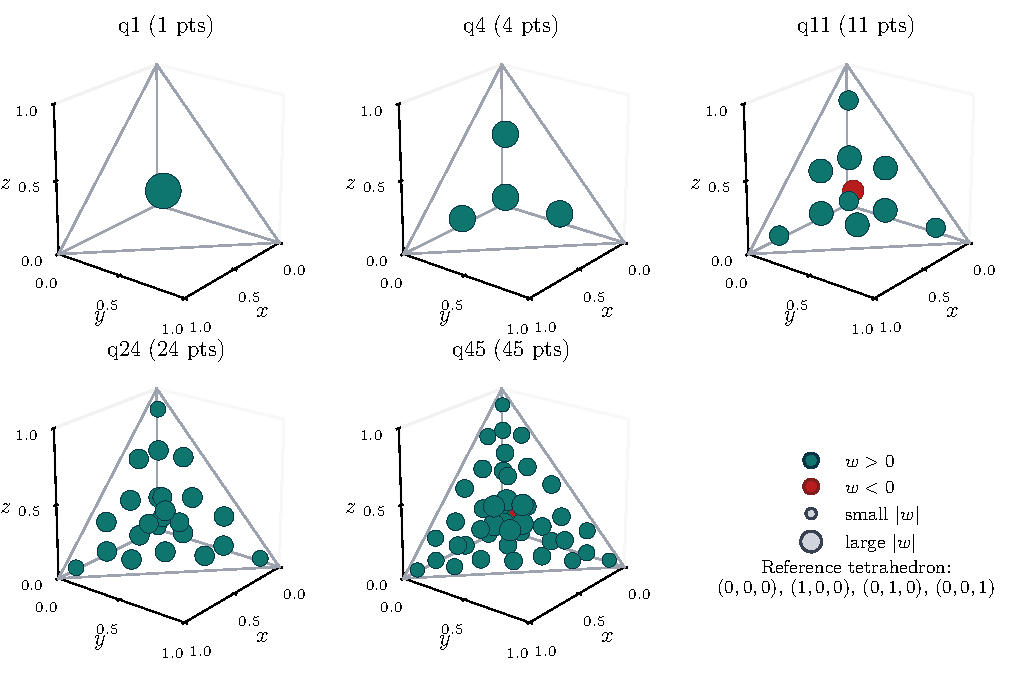
\includegraphics[width=\linewidth,height=0.60\textheight,keepaspectratio]{reference_tetra_quadratures.pdf}
\end{column}
\begin{column}{0.50\textwidth}
\begin{softbox}
\begin{itemize}
  \item The config and element helpers accept \code{P1}, \code{P2}, and \code{P4} on the public interface.
  \item The VTK export path supports \code{VTK\_LAGRANGE\_TETRAHEDRON} for \code{P4}, including correct node ordering.
  \item The postprocess layer adds pointwise deviatoric strain export for 3D \code{P4}, so the higher-order benchmark path can be visualised without dropping back to a low-order fallback.
  \item I treat this as a concrete architecture capability exercised by the benchmark in this talk, not as a blanket maturity claim for every 3D runner.
\end{itemize}
\end{softbox}
\end{column}
\end{columns}
\sourceline{\code{src/slope\_stability/core/elements.py}; \code{src/slope\_stability/postprocess/field\_exports.py}; \code{tests/test\_high\_order\_vtu\_export.py}}
\end{frame}

\begin{frame}{Mainline Versus Appendix Features}
\small
\begin{tabularx}{\textwidth}{p{0.31\textwidth}p{0.27\textwidth}Y}
\toprule
\textbf{Area} & \textbf{Mainline in this talk} & \textbf{Moved to appendix} \\
\midrule
3D mechanics path & \code{P4} heterogeneous SSR default & legacy global assembly paths \\
Preconditioning & \code{pmg\_shell} backend & BDDC, direct solves, built-in PETSc PMG variants \\
Continuation & indirect SSR, secant predictor, legacy omega control & direct SSR, fine-switch logic, streaming microsteps \\
Constitutive ownership & overlap mode & unique-owner recovery and legacy scatter variants \\
Speed study & committed \code{P2} controlled report & local exploratory scaling archives \\
\bottomrule
\end{tabularx}
\sourceline{\code{docs/petsc\_matlab\_map/chapters/mainline/*}; \code{docs/petsc\_matlab\_map/chapters/annex/*}}
\end{frame}

\SectionDivider{Unified Runners}{5}{9}

\begin{frame}{Benchmark Folder Contract}
\small
\begin{columns}[T,totalwidth=\textwidth]
\begin{column}{0.43\textwidth}
\begin{pseudobox}
benchmark\_name/\\
\ \ case.toml\\
\ \ run.sh\\
\ \ README.md\\
\ \ simulation.ipynb\\
\ \ visualisation.ipynb\\
\ \ artifacts/simulation/...
\end{pseudobox}
\end{column}
\begin{column}{0.53\textwidth}
\begin{softbox}
\begin{itemize}
  \item The folder, not the script file name, is the unit of execution and documentation.
  \item The same \code{case.toml} powers CLI runs, benchmark suites, generated notebooks, and export reconstruction.
  \item The folder layout is stable enough that automation can reason about every benchmark in a uniform way.
\end{itemize}
\end{softbox}
\end{column}
\end{columns}
\sourceline{\code{benchmarks/README.md}; \code{benchmarks/generate\_benchmark\_notebooks.py}}
\end{frame}

\begin{frame}{Public TOML Sections}
\small
\begin{tabularx}{\textwidth}{p{0.22\textwidth}Y}
\toprule
\textbf{Section} & \textbf{Purpose} \\
\midrule
\code{[problem]} & Case identity, analysis kind, dimension, variant, element type, mesh path, Davis choice, seepage flag \\
\code{[execution]} & Node ordering, MPI ownership mode, constitutive ownership mode, tangent kernel \\
\code{[continuation]} & Predictor, omega controller, target horizon, delta-lambda rules, fine-switch and warm-start controls \\
\code{[newton]} & Iteration limits, damping limits, stop criterion, stop tolerance \\
\code{[linear\_solver]} & Solver family, backend, matrix policy, rebuild policy, Hypre/GAMG/BDDC settings \\
\code{[seepage]} & Hydraulic solve tolerances and material conductivity data where relevant \\
\code{[export]} & Which standard outputs to write and how to name them \\
\code{[[materials]]} & Material rows in the same logical order as the MATLAB material table \\
\bottomrule
\end{tabularx}
\sourceline{\code{src/slope\_stability/core/run\_config.py}; \code{docs/config\_scheme\_3d.md}}
\end{frame}

\begin{frame}{Walkthrough Of The Architecture-Anchor \code{case.toml}}
\small
\begin{columns}[T,totalwidth=\textwidth]
\begin{column}{0.50\textwidth}
\begin{pseudobox}
\code{[problem]}\\
\code{case = "3d\_hetero\_ssr"}\\
\code{analysis = "ssr"}\\
\code{elem\_type = "P4"}\\
\code{mesh\_path = "../../meshes/...L1.msh"}\\[0.10cm]
\code{[execution]}\\
\code{node\_ordering = "block\_metis"}\\
\code{constitutive\_mode = "overlap"}\\[0.10cm]
\code{[linear\_solver]}\\
\code{pc\_backend = "pmg\_shell"}
\end{pseudobox}
\end{column}
\begin{column}{0.46\textwidth}
\begin{softbox}
\begin{itemize}
  \item This is enough to select the 3D SSR runner and the distributed architecture path I have been using as the anchor case.
  \item Notebook metadata lives in the same document, so the case also defines its 3D slice planes and display defaults.
  \item The config file is now the shortest route to understanding a benchmark.
\end{itemize}
\end{softbox}
\end{column}
\end{columns}
\sourceline{\code{benchmarks/slope\_stability\_3D\_hetero\_SSR\_default/case.toml}}
\end{frame}

\begin{frame}{Dispatch Through \code{run\_case\_from\_config}}
\small
\begin{columns}[T,totalwidth=\textwidth]
\begin{column}{0.52\textwidth}
\begin{pseudobox}
load config\\
$\rightarrow$ inspect \code{problem.case}\\
$\rightarrow$ map to one capture runner\\
$\rightarrow$ convert config fields to runner kwargs\\
$\rightarrow$ run the case\\
$\rightarrow$ rebuild case mesh for export\\
$\rightarrow$ write debug bundle, JSON, VTU
\end{pseudobox}
\end{column}
\begin{column}{0.44\textwidth}
\begin{softbox}
\begin{itemize}
  \item The dispatch layer is intentionally explicit rather than magical.
  \item Case-specific runners still exist, but the entrypoint surface is unified.
  \item This is the rewrite's replacement for choosing between many top-level MATLAB scripts.
\end{itemize}
\end{softbox}
\end{column}
\end{columns}
\sourceline{\code{src/slope\_stability/cli/run\_case\_from\_config.py}}
\end{frame}

\begin{frame}{How To Add A New Benchmark: Steps 1 To 3}
\small
\begin{enumerate}
  \item Create a new folder under \code{benchmarks/} with \code{case.toml}, \code{run.sh}, and \code{README.md}.
  \item Fill the \code{[benchmark]} block so the case has a title, MATLAB reference script, comparison kind, MPI rank default, and suite membership.
  \item Fill the runtime blocks: \code{[problem]}, \code{[execution]}, \code{[continuation]}, \code{[newton]}, \code{[linear\_solver]}, and optionally \code{[seepage]}, \code{[export]}, \code{[[materials]]}.
\end{enumerate}
\vspace{0.18cm}
\begin{callout}
If the case belongs to an existing mesh family, reusing the mesh-family definition can remove the need to restate the material table in the benchmark itself.
\end{callout}
\sourceline{\code{benchmarks/README.md}; \code{src/slope\_stability/problem\_assets.py}}
\end{frame}

\begin{frame}{How To Add A New Benchmark: Steps 4 To 5}
\small
\begin{enumerate}
  \item Add an optional \code{[notebook]} block so the generated simulation and visualisation notebooks know the family, display backend, P4 surface subdivision, decimation, and slice planes.
  \item Run the case once so \code{artifacts/simulation/} exists and the standard outputs can be reused by notebooks and postprocessing.
\end{enumerate}
\vspace{0.18cm}
\begin{softbox}
\miniheading{Checklist before you call it ``done''}
\begin{itemize}
  \item Does \code{run.sh} call the same config that the notebooks use?
  \item Does the README describe the case without hiding the runtime contract?
  \item Are the exported fields sufficient for the visualisation family you selected?
  \item If it belongs in the parity suite, is \code{[benchmark].suite = true} set intentionally?
\end{itemize}
\end{softbox}
\sourceline{\code{benchmarks/generate\_benchmark\_notebooks.py}; \code{benchmarks/prepare\_committed\_notebook\_artifacts.py}}
\end{frame}

\SectionDivider{Unified Visualisation}{6}{9}

\begin{frame}{Unified Visualisation Pipeline}
\small
\begin{pseudobox}
solve case\\
$\rightarrow$ write \code{final\_solution.vtu} + debug bundle + history JSON\\
$\rightarrow$ rebuild case mesh from config\\
$\rightarrow$ build standard field exports\\
$\rightarrow$ generated notebooks / PyVista / ParaView consume the same files
\end{pseudobox}
\vspace{0.20cm}
\begin{columns}[T,totalwidth=\textwidth]
\begin{column}{0.49\textwidth}
\begin{softbox}
\miniheading{Key rewrite helpers}
\begin{itemize}
  \item \code{postprocess/case\_mesh.py}
  \item \code{postprocess/field\_exports.py}
  \item \code{benchmarks/notebook\_support.py}
\end{itemize}
\end{softbox}
\end{column}
\begin{column}{0.49\textwidth}
\begin{softbox}
\miniheading{What that buys}
\begin{itemize}
  \item one mesh reconstruction surface
  \item one field naming surface
  \item one notebook generation surface
  \item one export surface for external viewers
\end{itemize}
\end{softbox}
\end{column}
\end{columns}
\sourceline{\code{src/slope\_stability/postprocess/case\_mesh.py}; \code{src/slope\_stability/postprocess/field\_exports.py}; \code{benchmarks/notebook\_support.py}}
\end{frame}

\begin{frame}{PETSc 3D Views: Geometry And Warped Displacement}
\small
\begin{columns}[T,totalwidth=\textwidth]
\begin{column}{0.49\textwidth}
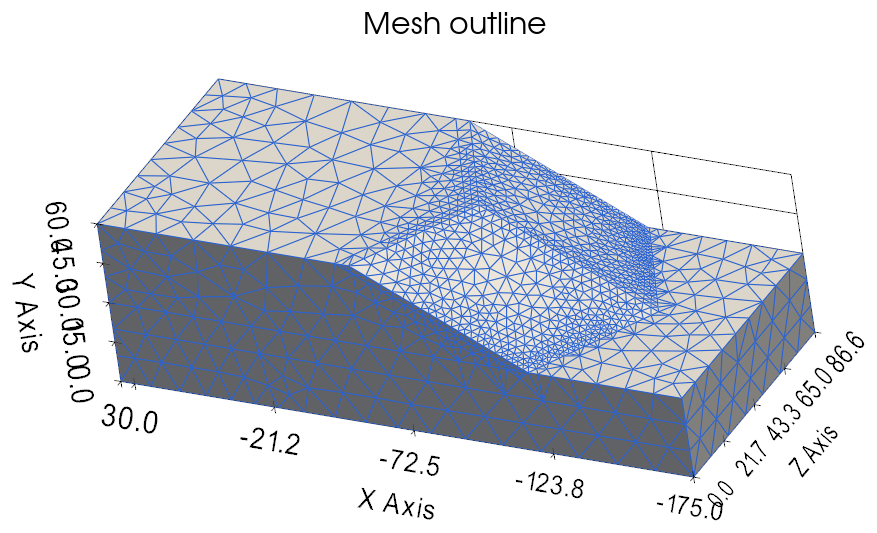
\includegraphics[width=\linewidth,height=0.48\textheight,keepaspectratio]{petsc_geometry_current.png}
\end{column}
\begin{column}{0.49\textwidth}
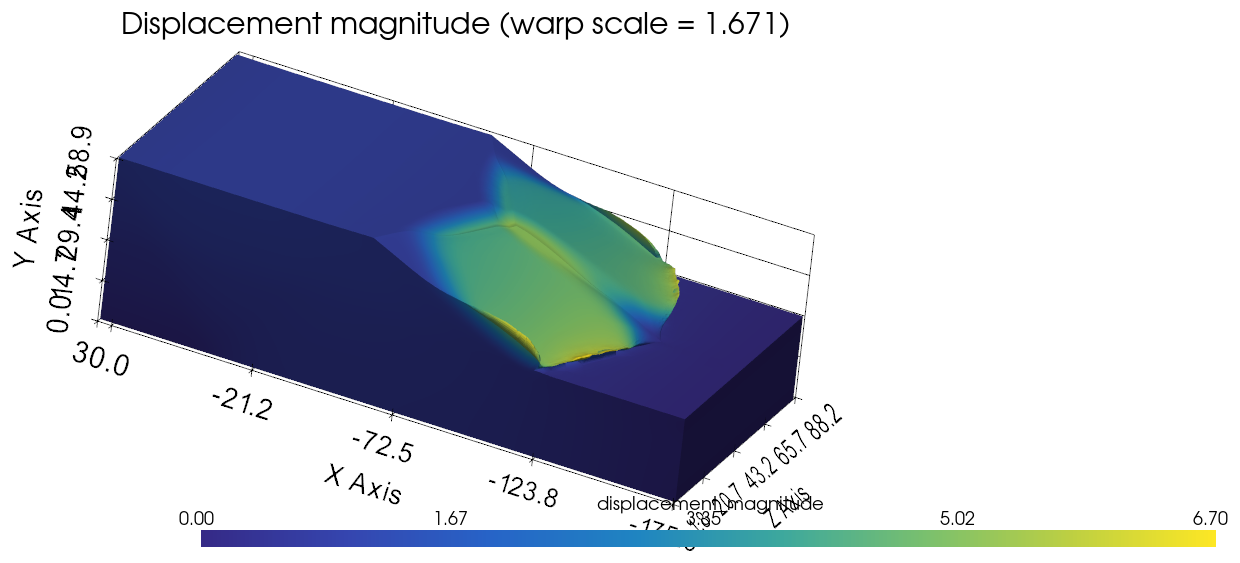
\includegraphics[width=\linewidth,height=0.48\textheight,keepaspectratio]{petsc_displacement_current.png}
\end{column}
\end{columns}
\vspace{0.12cm}
\begin{softbox}
\begin{itemize}
  \item Both panels are taken from the default indirect 3D SSR visualisation notebook path.
  \item On the left I show the mesh-outline view that makes the local refinement pattern immediately visible.
  \item On the right I show the warped displacement view from the same benchmark and the same exported solution bundle.
\end{itemize}
\end{softbox}
\end{frame}

\begin{frame}{PETSc Localisation Surface And Top-View Slices}
\small
\begin{columns}[T,totalwidth=\textwidth]
\begin{column}{0.42\textwidth}
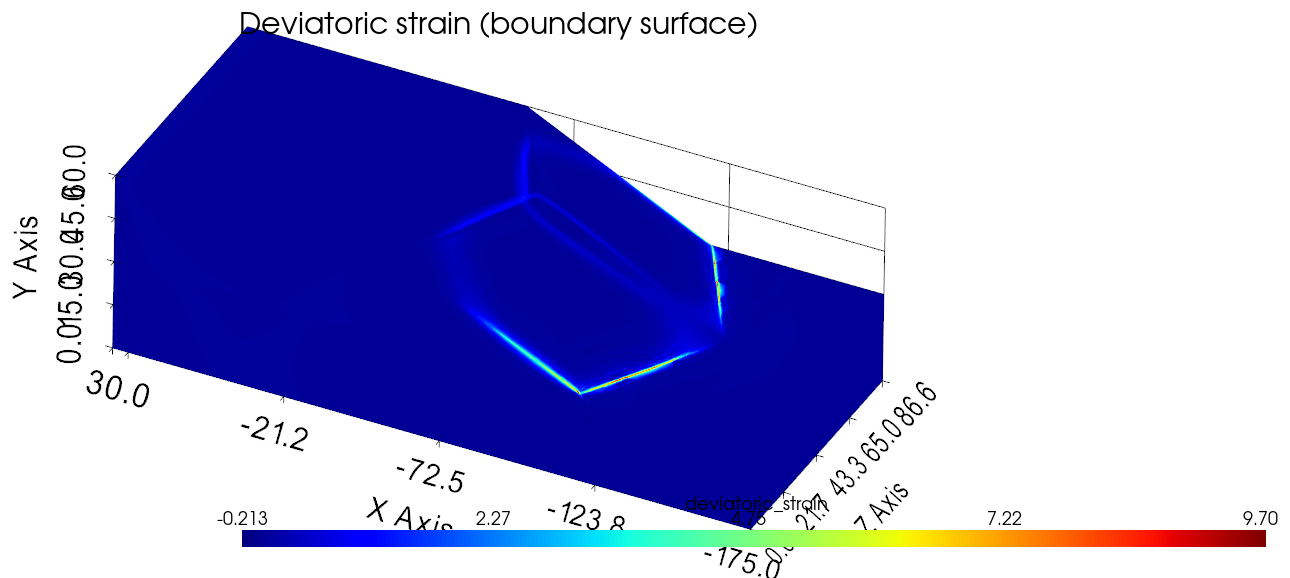
\includegraphics[width=\linewidth,height=0.46\textheight,keepaspectratio]{petsc_deviatoric_surface_current.png}
\end{column}
\begin{column}{0.55\textwidth}
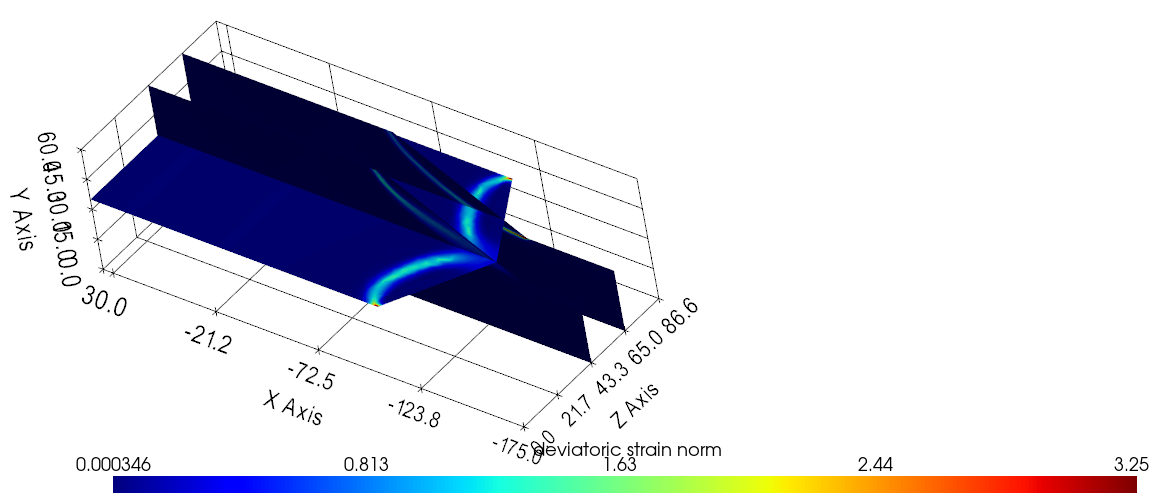
\includegraphics[width=\linewidth,height=0.41\textheight,keepaspectratio]{petsc_slices_current.png}
\end{column}
\end{columns}
\vspace{0.16cm}
\begin{softbox}
\begin{itemize}
  \item Both panels come from the same default indirect visualisation path and the same exported \code{deviatoric\_strain} field.
  \item The 3D panel keeps the notebook-style full boundary-surface view that the authors are already used to reading.
  \item The slice panel stays a real top-view cut product at the benchmark-configured planes, with the same capped warm-to-cool scale used in the 3D deviatoric view shown on the left.
\end{itemize}
\end{softbox}
\end{frame}

\begin{frame}{MATLAB And PETSc Reach Similar Slice Products Through Different Workflows}
\small
\begin{columns}[T,totalwidth=\textwidth]
\begin{column}{0.49\textwidth}
\miniheading{MATLAB}
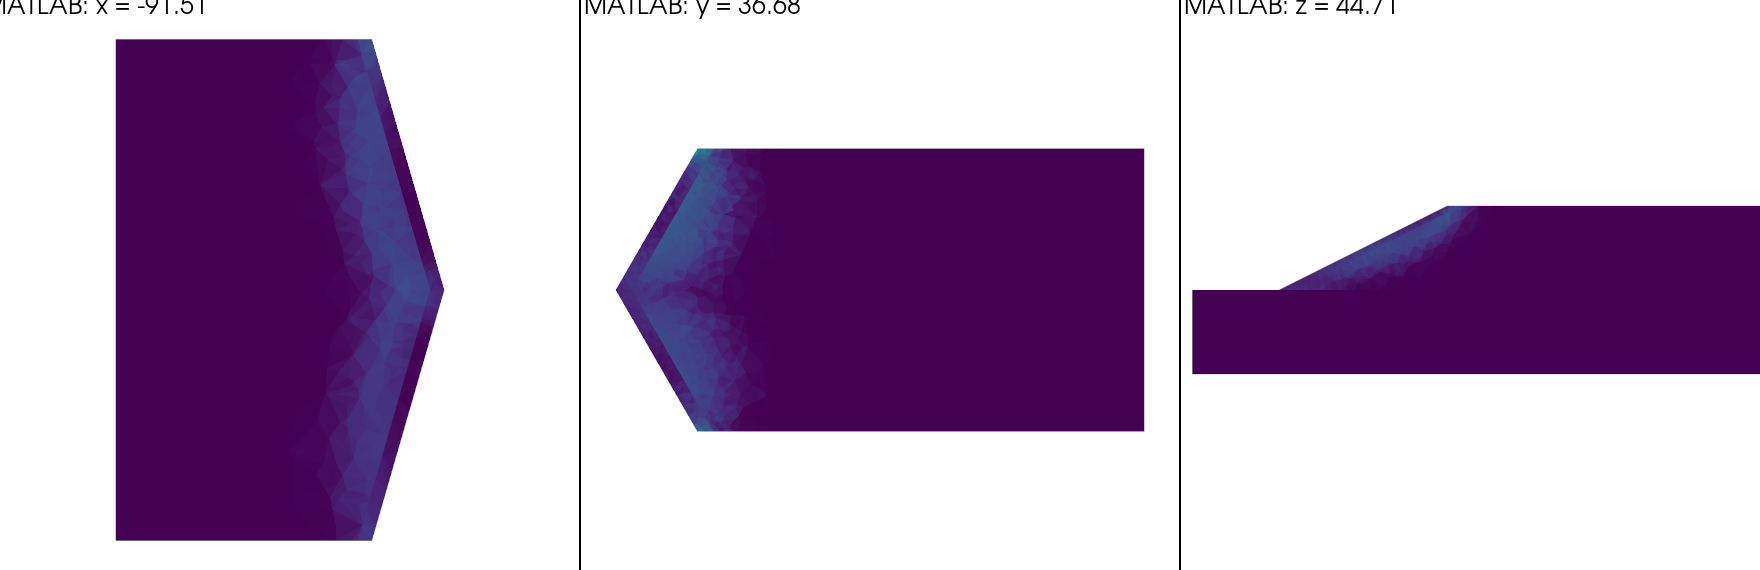
\includegraphics[width=\linewidth,height=0.38\textheight,keepaspectratio]{matlab_slices_present.png}
\end{column}
\begin{column}{0.49\textwidth}
\miniheading{PETSc rewrite}
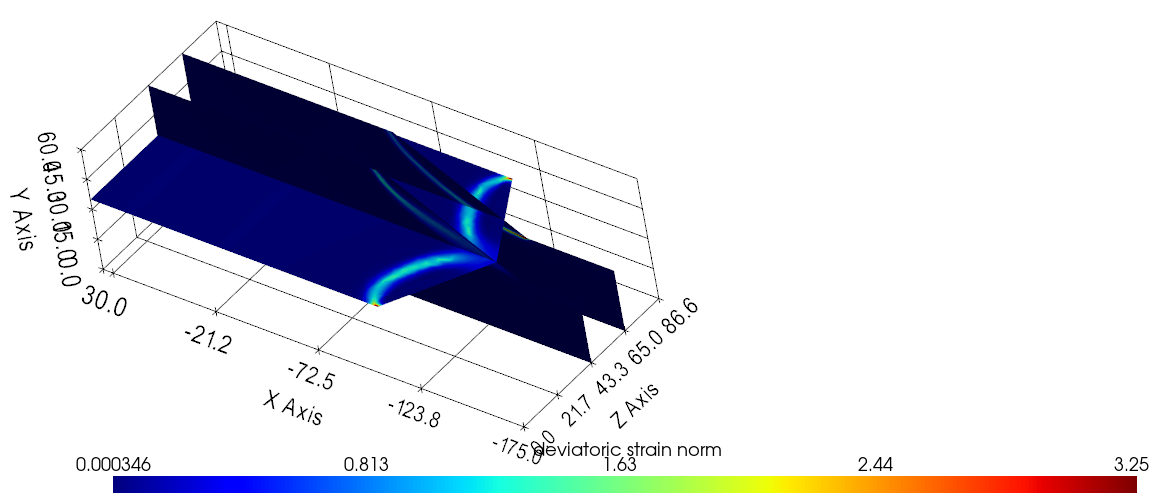
\includegraphics[width=\linewidth,height=0.38\textheight,keepaspectratio]{petsc_slices_current.png}
\end{column}
\end{columns}
\vspace{0.14cm}
\begin{callout}
What changes for me is not whether I can inspect the same slice family. What changes is where the slice product comes from. MATLAB builds it in the case script; the rewrite rebuilds it from shared exports and shared notebook support.
\end{callout}
\end{frame}

\begin{frame}{Reuse In PyVista And ParaView}
\small
\begin{tabularx}{\textwidth}{p{0.26\textwidth}Y}
\toprule
\textbf{Output} & \textbf{Why it matters} \\
\midrule
\code{final\_solution.vtu} & Standard mesh plus field export for PyVista, meshio, and ParaView \\
\code{run\_debug.h5} & Dense debug bundle for deeper analysis and reproducibility \\
\code{continuation\_history.json} & Lightweight branch history for dashboards and comparisons \\
\code{resolved\_config.toml} & Exact runtime config that produced the outputs \\
\bottomrule
\end{tabularx}
\vspace{0.18cm}
\begin{softbox}
\begin{itemize}
  \item For 3D cases, the postprocess layer can rebuild the case mesh, attach displacement, pore pressure, saturation, and deviatoric strain, and then hand those fields to PyVista viewers or save them for ParaView.
  \item That is a much more uniform story than ``run the script and hope the workspace still contains the right arrays for plotting''.
\end{itemize}
\end{softbox}
\sourceline{\code{README.md}; \code{src/slope\_stability/postprocess/field\_exports.py}; \code{benchmarks/notebook\_support.py}}
\end{frame}

\SectionDivider{Unified Meshes}{7}{9}

\begin{frame}{MATLAB Mesh Handling And Element Degree Are Entangled}
\small
\begin{tabularx}{\textwidth}{p{0.28\textwidth}p{0.27\textwidth}Y}
\toprule
\textbf{Question} & \textbf{MATLAB answer} & \textbf{Consequence} \\
\midrule
Which file do I load? & Usually a degree-specific loader & Mesh storage and FE order drift together \\
How do I get P4 support? & Build new midpoint utilities and matching assumptions & Higher order grows sideways by utility proliferation \\
Where are materials and BC labels interpreted? & Inside the case loader path & Harder to reuse across benchmark families \\
Where does the free mask come from? & Loader-specific face conventions & Less separation between geometry and solve policy \\
\bottomrule
\end{tabularx}
\sourceline{\code{slope\_stability\_matlab/+MESH/load\_mesh\_P2.m}; \code{slope\_stability\_matlab/+MESH/midpoints\_P4.m}}
\end{frame}

\begin{frame}{PETSc Mesh Families Carry Their Own Metadata}
\small
\begin{columns}[T,totalwidth=\textwidth]
\begin{column}{0.52\textwidth}
\begin{pseudobox}
\code{DEFINITION = \{}\\
\code{  "name": "3d\_hetero\_ssr",}\\
\code{  "storage": "gmsh\_tet4\_physical\_groups",}\\
\code{  "default\_mesh": "SSR\_hetero\_ada\_L1.msh",}\\
\code{  "dirichlet\_labels": \{...\},}\\
\code{  "materials": [ ... ]}\\
\code{\}}
\end{pseudobox}
\end{column}
\begin{column}{0.44\textwidth}
\begin{softbox}
\begin{itemize}
  \item Each mesh family can declare canonical storage, default files, boundary labels, and material rows.
  \item The benchmark can then reference the family by mesh path and optionally inherit its material table.
  \item This makes the mesh family a reusable asset, not just a raw file on disk.
\end{itemize}
\end{softbox}
\end{column}
\end{columns}
\sourceline{\code{meshes/3d\_hetero\_ssr/definition.py}; \code{src/slope\_stability/problem\_assets.py}}
\end{frame}

\begin{frame}{Canonical Gmsh Tet4 Storage With Loader-Side Elevation}
\small
\begin{columns}[T,totalwidth=\textwidth]
\begin{column}{0.53\textwidth}
\begin{pseudobox}
canonical family mesh\\
$\rightarrow$ Gmsh tet4 + physical groups\\
$\rightarrow$ loader reads boundary/material tags\\
$\rightarrow$ solver requests \code{P1}, \code{P2}, or \code{P4}\\
$\rightarrow$ loader elevates connectivity as needed\\
$\rightarrow$ exports preserve the chosen FE order
\end{pseudobox}
\end{column}
\begin{column}{0.43\textwidth}
\begin{softbox}
\begin{itemize}
  \item The family file does not need to be duplicated per degree.
  \item The rewrite can keep one canonical geometry/material definition while the solver selects its FE degree.
  \item This is the cleanest contrast to the MATLAB P2-only HDF5 path.
\end{itemize}
\end{softbox}
\end{column}
\end{columns}
\sourceline{\code{src/slope\_stability/io.py}; \code{src/slope\_stability/mesh/loader.py}; \code{README.md}}
\end{frame}

\begin{frame}{Mesh Family And \code{elem\_type} Are Now Separate Concepts}
\small
\begin{tabularx}{\textwidth}{p{0.30\textwidth}p{0.25\textwidth}Y}
\toprule
\textbf{Concept} & \textbf{Where it lives} & \textbf{Meaning} \\
\midrule
Mesh family & \code{meshes/*/definition.py} + mesh files & Geometry, physical tags, default material metadata \\
\code{problem.mesh\_path} & \code{case.toml} & Which family member or external mesh file to load \\
\code{problem.elem\_type} & \code{case.toml} & Which FE degree the runtime should use on that mesh \\
Export cell type & \code{core/elements.py} & How the chosen FE degree is written back to VTU \\
\bottomrule
\end{tabularx}
\vspace{0.18cm}
\begin{callout}
This is the core 3D mesh design change: \term{geometry/material family selection} and \term{finite-element degree selection} are no longer the same decision.
\end{callout}
\sourceline{\code{src/slope\_stability/core/elements.py}; \code{src/slope\_stability/problem\_assets.py}; \code{docs/config\_case\_matrix.md}}
\end{frame}

\begin{frame}{Boundary Tags, Material Tags, And Reordering Stay Explicit}
\small
\begin{columns}[T,totalwidth=\textwidth]
\begin{column}{0.32\textwidth}
\MetricTile{Boundary labels}{
Mesh-family metadata declares which physical labels correspond to constrained \(x\), \(y\), and \(z\) directions.
}
\end{column}
\begin{column}{0.32\textwidth}
\MetricTile{Material identifiers}{
Element-wise material ids stay attached to the mesh and can be expanded into integration-point rows later.
}
\end{column}
\begin{column}{0.32\textwidth}
\MetricTile{Node reorder}{
The same mesh can then be reordered for ownership without losing its physical meaning.
}
\end{column}
\end{columns}
\vspace{0.20cm}
\begin{softbox}
The rewrite does not hide physics labels behind generic partitioning. It keeps labels explicit, then reorders the discrete system around them.
\end{softbox}
\sourceline{\code{meshes/3d\_hetero\_ssr/definition.py}; \code{src/slope\_stability/mesh/reorder.py}; \code{docs/petsc\_matlab\_map/chapters/mainline/02\_mesh\_materials\_load.tex}}
\end{frame}

\SectionDivider{Speed Comparison}{8}{9}

\begin{frame}{Before I Quote Runtimes, Here Is The Locked Study Protocol}
\small
\begin{softbox}
\begin{itemize}
  \item The committed PETSc-vs-MATLAB performance report uses indirect SSR only and \code{P2} elements only.
  \item PETSc runs use \code{mpirun -n 8} with \code{OMP\_NUM\_THREADS = 1}.
  \item MATLAB runs use \code{OMP\_NUM\_THREADS = 8} with the BoomerAMG MATLAB path on 8 threads.
  \item The three primary cases are homogeneous 3D SSR, heterogeneous 3D SSR, and heterogeneous 3D seepage SSR.
  \item The study is sequential and normalised into CSV before figures and tables are built.
\end{itemize}
\end{softbox}
\vspace{0.18cm}
\begin{callout}
The study answers ``how does the committed P2 PETSc implementation compare under this controlled protocol?'' It does \textbf{not} directly answer ``how fast is the current default P4 architecture path?''.
\end{callout}
\datasourceline{\code{docs/petsc\_matlab\_performance\_comparison}: README and main LaTeX report}
\end{frame}

\begin{frame}{Locked P2 Study: Headline View Across The Three Cases}
\small
\begin{tabularx}{\textwidth}{p{0.27\textwidth}p{0.16\textwidth}p{0.15\textwidth}Y}
\toprule
\textbf{Case} & \textbf{Levels} & \textbf{M/P gap} & \textbf{Headline} \\
\midrule
Homogeneous 3D SSR & L1 to L4 & \(1.24\times\) to \(3.47\times\) & PETSc pulls further ahead as the dry mesh ladder grows. \\
Heterogeneous 3D SSR & L1 to L4 & \(1.35\times\) to \(3.08\times\) & Same trend on the dry case closest to the architecture anchor. \\
Heterogeneous 3D seepage SSR & \code{concave\_L2} only & \(2.02\times\) & Positive completed level, but the next level remains part of the reported limitation. \\
\bottomrule
\end{tabularx}
\datasourceline{committed \code{P2} study generated tables in \code{docs/petsc\_matlab\_performance\_comparison/generated}}
\end{frame}

\begin{frame}{Homogeneous 3D SSR: PETSc Pulls Ahead As The Mesh Grows}
\small
\begin{columns}[T,totalwidth=\textwidth]
\begin{column}{0.49\textwidth}
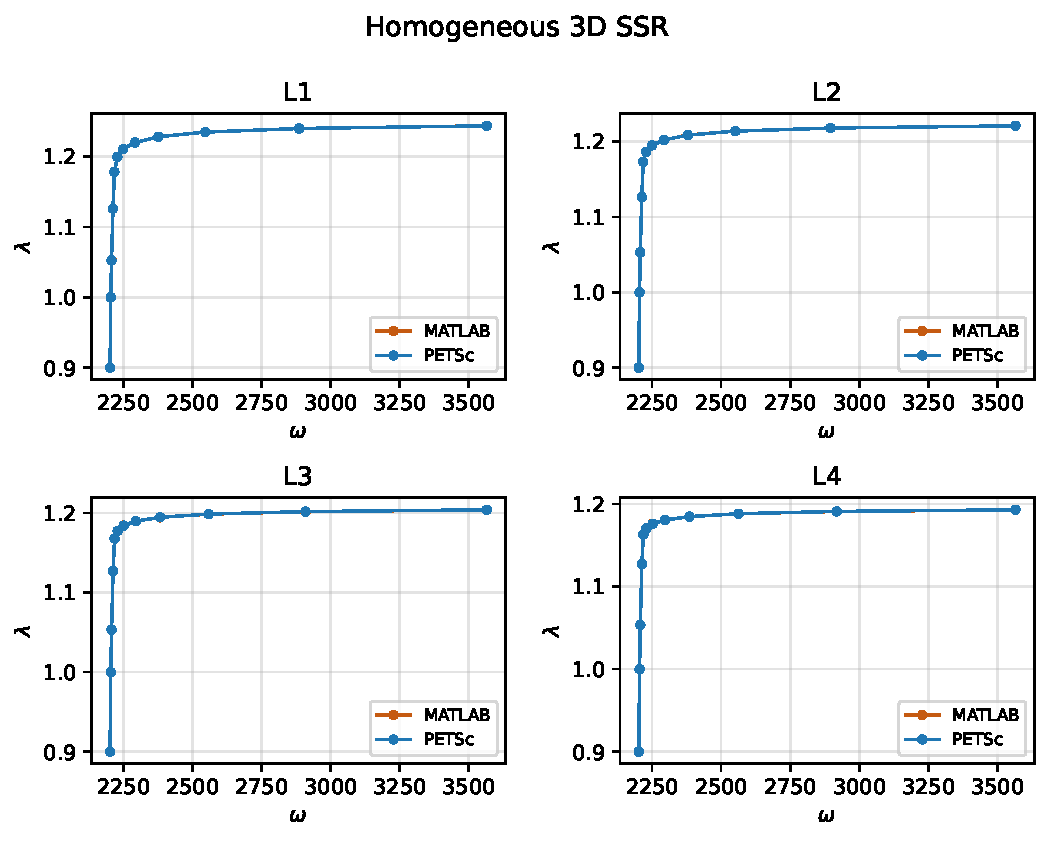
\includegraphics[width=\linewidth,height=0.50\textheight,keepaspectratio]{homo_3d_continuation.pdf}
\end{column}
\begin{column}{0.49\textwidth}
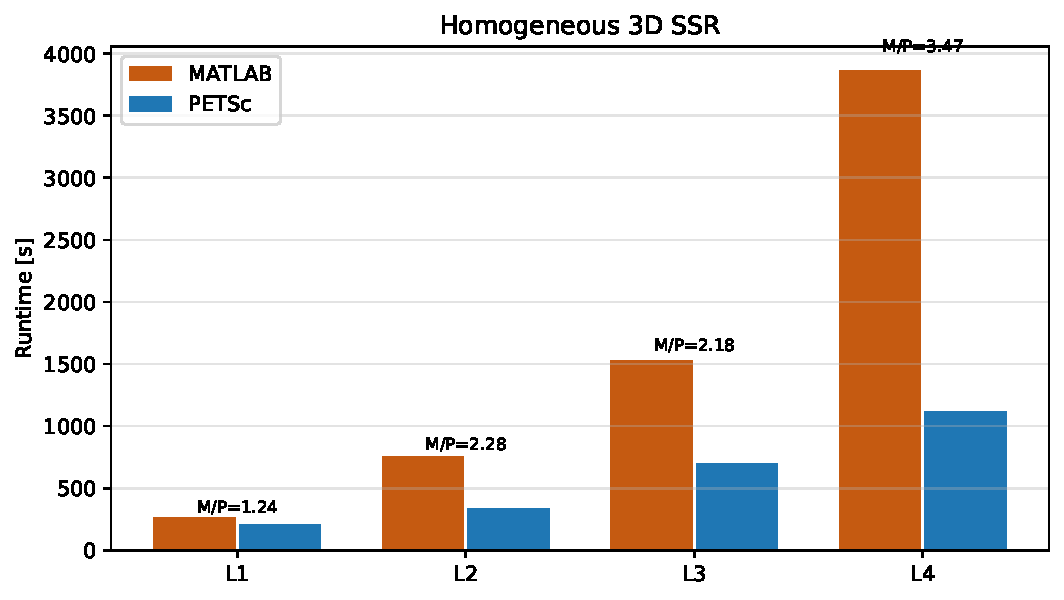
\includegraphics[width=\linewidth,height=0.50\textheight,keepaspectratio]{homo_3d_timings.pdf}
\end{column}
\end{columns}
\vspace{0.14cm}
\begin{softbox}
\begin{itemize}
  \item PETSc runtime goes from \(210.5\) s at L1 to \(1115.2\) s at L4.
  \item MATLAB runtime goes from \(261.8\) s at L1 to \(3865.1\) s at L4.
  \item The MATLAB-over-PETSc ratio grows from \(1.24\times\) to \(3.47\times\).
\end{itemize}
\end{softbox}
\datasourceline{\code{presentation\_petsc\_rewrite/assets}: homogeneous 3D continuation and timings from the committed study}
\end{frame}

\begin{frame}{Heterogeneous 3D SSR: Same Trend, Stronger Advantage On Larger Levels}
\small
\begin{columns}[T,totalwidth=\textwidth]
\begin{column}{0.49\textwidth}
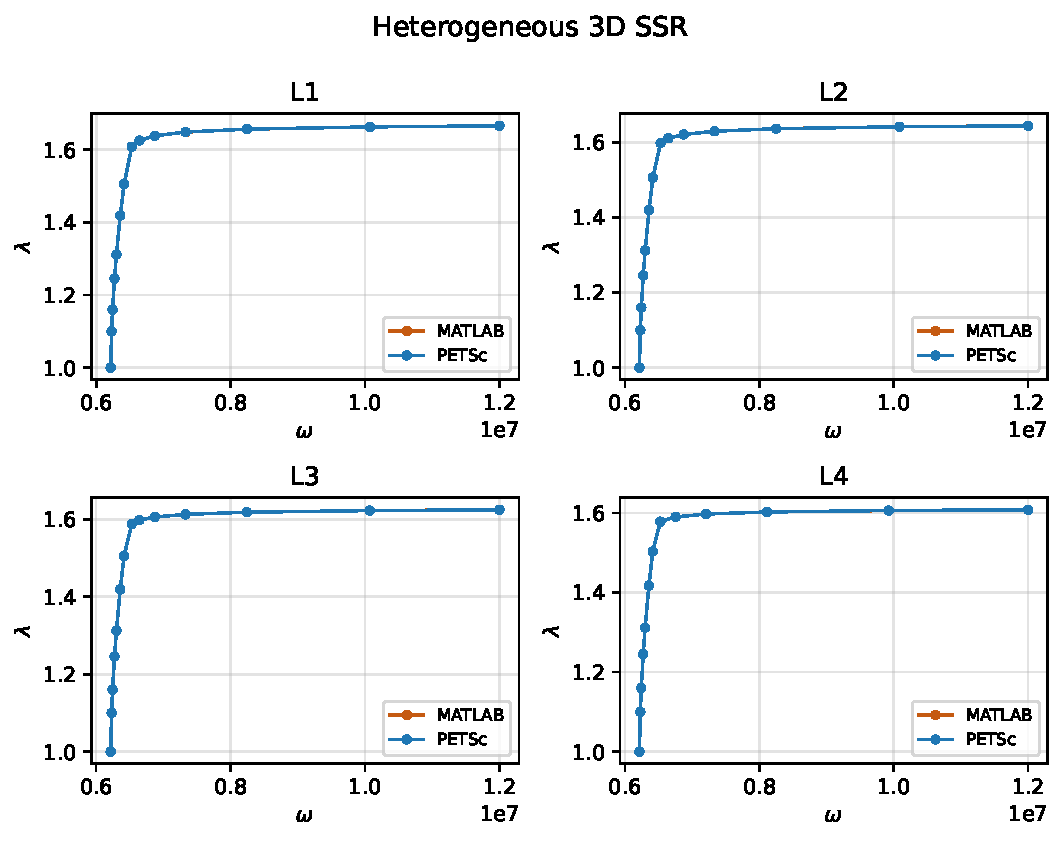
\includegraphics[width=\linewidth,height=0.50\textheight,keepaspectratio]{hetero_3d_continuation.pdf}
\end{column}
\begin{column}{0.49\textwidth}
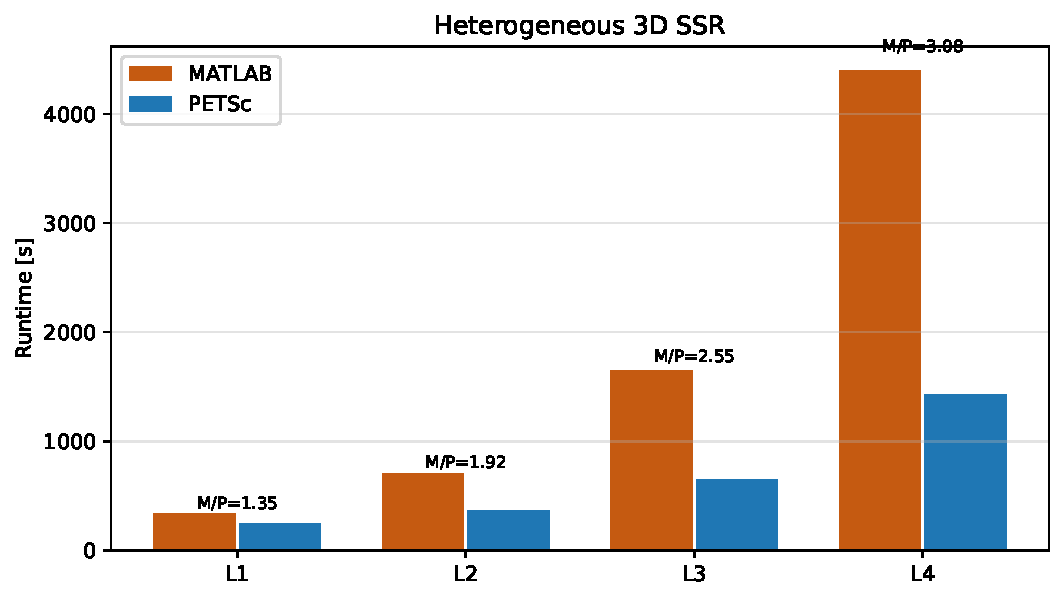
\includegraphics[width=\linewidth,height=0.50\textheight,keepaspectratio]{hetero_3d_timings.pdf}
\end{column}
\end{columns}
\vspace{0.14cm}
\begin{softbox}
\begin{itemize}
  \item PETSc runtime grows from \(247.3\) s at L1 to \(1430.2\) s at L4.
  \item MATLAB runtime grows from \(334.2\) s at L1 to \(4399.1\) s at L4.
  \item The MATLAB-over-PETSc ratio grows from \(1.35\times\) to \(3.08\times\).
\end{itemize}
\end{softbox}
\datasourceline{\code{presentation\_petsc\_rewrite/assets}: heterogeneous 3D continuation and timings from the committed study}
\end{frame}

\begin{frame}{Seepage 3D SSR: Only One Level Completed Under The Locked Protocol}
\small
\begin{columns}[T,totalwidth=\textwidth]
\begin{column}{0.49\textwidth}
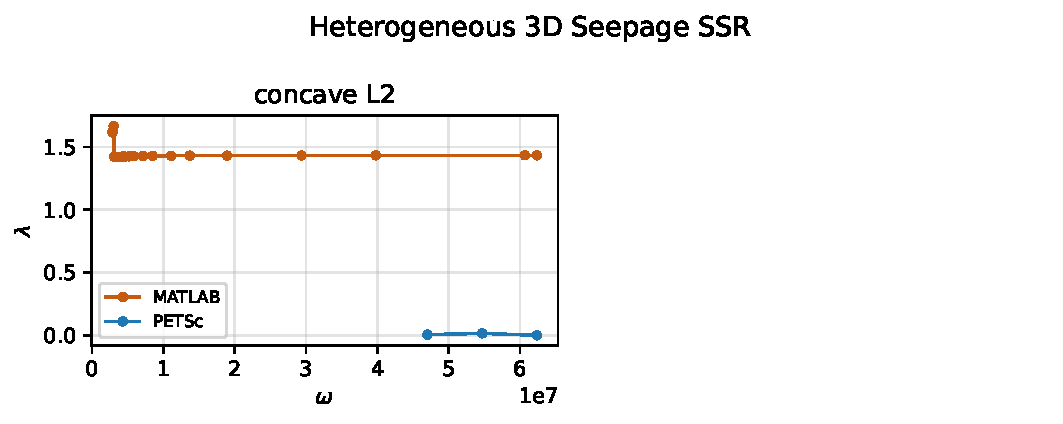
\includegraphics[width=\linewidth,height=0.50\textheight,keepaspectratio]{seepage_3d_continuation.pdf}
\end{column}
\begin{column}{0.49\textwidth}
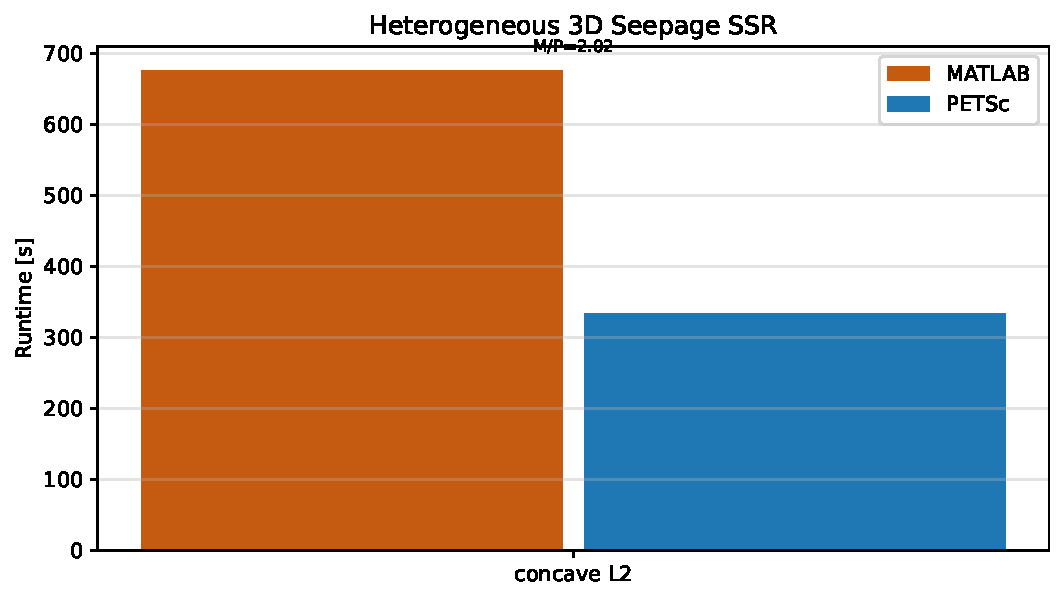
\includegraphics[width=\linewidth,height=0.50\textheight,keepaspectratio]{seepage_3d_timings.pdf}
\end{column}
\end{columns}
\vspace{0.14cm}
\begin{softbox}
\begin{itemize}
  \item On \code{concave\_L2}, PETSc finished in \(334.1\) s and MATLAB in \(676.3\) s, a \(2.02\times\) advantage.
  \item Only this level completed under the committed mixed PMG-shell seepage study protocol.
  \item The next seepage level failed on the PETSc side after hierarchy construction and outer-solver setup, so the report deliberately stops at the completed comparison.
\end{itemize}
\end{softbox}
\datasourceline{\code{presentation\_petsc\_rewrite/assets}: seepage 3D continuation and timings from the committed study}
\end{frame}

\begin{frame}{Additional Speedup Gain: The Delta-Lambda Stop Rule}
\small
\begin{columns}[T,totalwidth=\textwidth]
\begin{column}{0.49\textwidth}
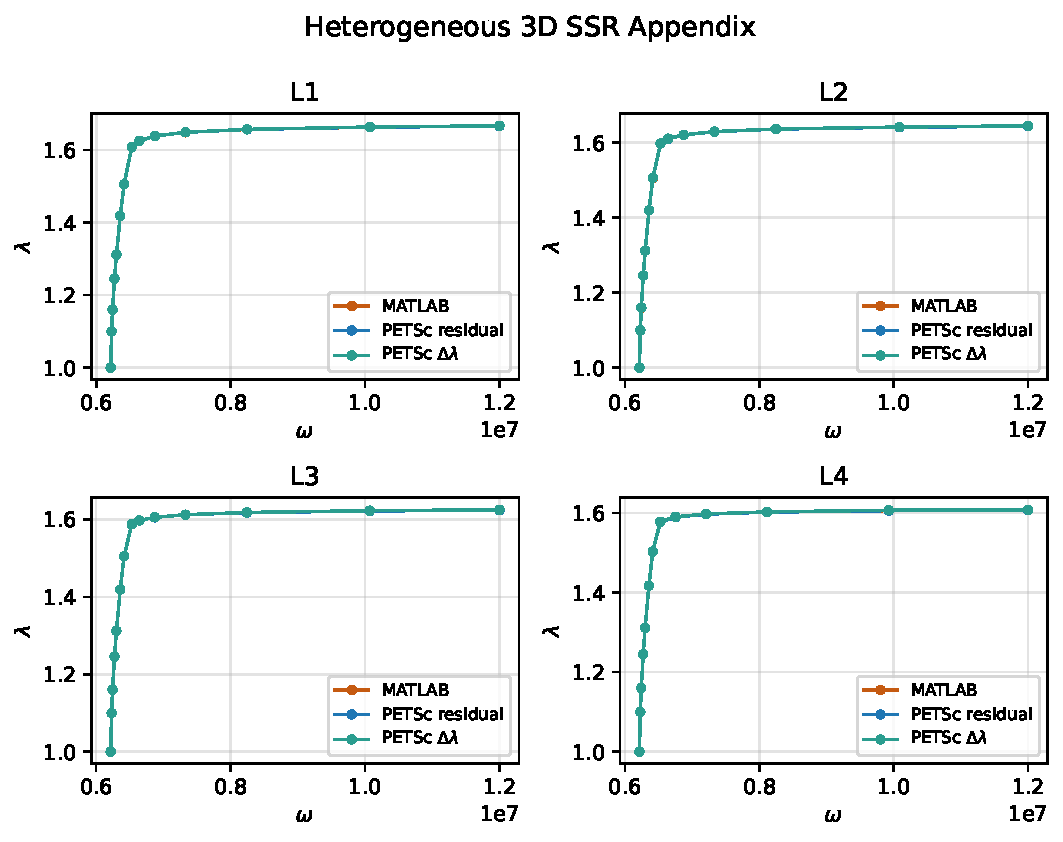
\includegraphics[width=\linewidth,height=0.40\textheight,keepaspectratio]{hetero_3d_delta_lambda_continuation.pdf}
\end{column}
\begin{column}{0.49\textwidth}
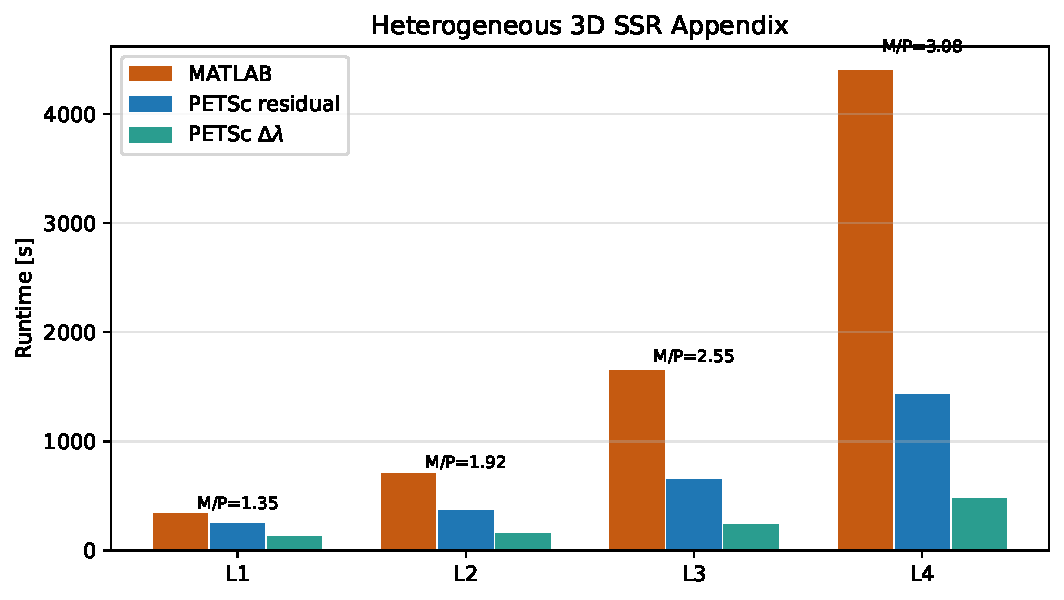
\includegraphics[width=\linewidth,height=0.40\textheight,keepaspectratio]{hetero_3d_delta_lambda_timings.pdf}
\end{column}
\end{columns}
\vspace{0.10cm}
\begin{columns}[T,totalwidth=\textwidth]
\begin{column}{0.52\textwidth}
\begin{softbox}
\begin{itemize}
  \item On the same heterogeneous dry study, the \(\Delta\lambda\) stop rule is \(2.0\times\) faster than the residual baseline at L1 and \(3.0\times\) faster at L4.
  \item Against MATLAB, that pushes the gap from \(2.7\times\) at L1 to \(9.3\times\) at L4.
\end{itemize}
\end{softbox}
\end{column}
\begin{column}{0.44\textwidth}
\begin{callout}
I treat this as a controlled ``other speedup gain'' slide. The study branch stays the same; only the stop policy changes.
\end{callout}
\end{column}
\end{columns}
\datasourceline{\code{docs/petsc\_matlab\_performance\_comparison}: delta-lambda figures and generated table}
\end{frame}

\SectionDivider{Close}{9}{9}

\begin{frame}{Key Takeaways For The Original MATLAB Authors}
\small
\begin{softbox}
\begin{itemize}
  \item The rewrite preserves the familiar nonlinear story, but it changes how responsibilities are packaged and where data lives.
  \item Config files and mesh-family metadata replace large parts of the old top-level script surface.
  \item Owned-row distributed assembly and explicit solver backends are the main structural changes that enabled parallel capabilities.
  \item Standard exports and notebook tooling replace much of the old case-local visualisation burden.
  \item The committed P2 speed study already shows clear PETSc advantages on the main 3D dry cases, while also documenting current seepage limitations honestly.
\end{itemize}
\end{softbox}
\end{frame}

\begin{frame}{Recommended Reading Order For New Contributors}
\small
\begin{tabularx}{\textwidth}{p{0.28\textwidth}Y}
\toprule
\textbf{If your question is...} & \textbf{Start here} \\
\midrule
How does the default \code{P4} architecture benchmark run end to end? & \code{benchmarks/slope\_stability\_3D\_hetero\_SSR\_default/case.toml}, then \code{cli/run\_case\_from\_config.py}, then \code{cli/run\_3D\_hetero\_SSR\_capture.py} \\
How does the old MATLAB logic map onto the rewrite? & \code{docs/petsc\_matlab\_map/*} \\
How are mesh family and materials declared now? & \code{meshes/*/definition.py} plus \code{problem\_assets.py} \\
How are fields exported and visualised? & \code{postprocess/*}, \code{benchmarks/notebook\_support.py} \\
What performance claims are currently documented? & \code{docs/petsc\_matlab\_performance\_comparison/*} \\
\bottomrule
\end{tabularx}
\end{frame}

\begin{frame}{Final Summary}
\small
\begin{columns}[T,totalwidth=\textwidth]
\begin{column}{0.32\textwidth}
\MetricTile{What stayed the same}{
SSR, Newton, constitutive reduction, and the benchmark families remain recognisable to the MATLAB authors.
}
\end{column}
\begin{column}{0.32\textwidth}
\MetricTile{What changed}{
Configuration, ownership-aware assembly, solver backend separation, standard exports, and shared notebooks became first-class interfaces.
}
\end{column}
\begin{column}{0.32\textwidth}
\MetricTile{What to discuss next}{
Which paths should be treated as production defaults, which appendix branches deserve more work, and where parity versus performance should be prioritised next.
}
\end{column}
\end{columns}
\end{frame}

\appendix
\AppendixDivider{Optional Paths, Caveats, And Additional Reading}

\begin{frame}{Architecture Mainline Versus Performance Study Protocol}
\small
\begin{tabularx}{\textwidth}{p{0.28\textwidth}p{0.26\textwidth}Y}
\toprule
\textbf{Question} & \textbf{Architecture mainline} & \textbf{Committed performance study} \\
\midrule
Purpose & Explain the current rewrite structure & Compare PETSc and MATLAB under one locked protocol \\
Case anchor & \code{default P4 benchmark} & \code{committed P2 report} \\
Element degree & \code{P4} default path & \code{P2} only \\
Solver backend focus & \code{pmg\_shell}, owned-row path & PETSc MPI-8 versus MATLAB OMP-8 \\
What it proves & How the rewrite is structured today & How one committed PETSc branch compares numerically and in runtime \\
\bottomrule
\end{tabularx}
\end{frame}

\begin{frame}{Optional And Inactive Paths Present In The Repository}
\small
\begin{softbox}
\begin{itemize}
  \item Direct SSR and LL continuation remain present and runnable for selected cases.
  \item BDDC, Hypre, GAMG, and multiple PMG variants all exist as selectable branches.
  \item Different constitutive ownership modes remain available beyond the overlap mainline.
  \item The map document keeps these paths in its annex so they do not distort the default-reading story.
\end{itemize}
\end{softbox}
\sourceline{\code{docs/petsc\_matlab\_map/chapters/annex/*}; \code{src/slope\_stability/continuation/*}; \code{src/slope\_stability/linear/*}}
\end{frame}

\begin{frame}{Global Assembly And The Legacy Tangent Kernel}
\small
\begin{tabularx}{\textwidth}{p{0.26\textwidth}p{0.26\textwidth}Y}
\toprule
\textbf{Path} & \textbf{Still present?} & \textbf{Why it is not the default story} \\
\midrule
Global \code{B' D B} rebuild & yes & It matches the old MATLAB intuition better, but it is not the normal owned-row PMG route \\
Legacy tangent kernel & yes & Kept for comparison and fallback, but the \code{rows} kernel is the production default for the mainline path \\
Legacy scatter-style assembly & yes & Appendix material now that overlap-owned assembly is the default architectural choice \\
\bottomrule
\end{tabularx}
\sourceline{\code{docs/petsc\_matlab\_map/chapters/annex/05\_tangent\_assembly.tex}; \code{src/slope\_stability/fem/distributed\_tangent.py}}
\end{frame}

\begin{frame}{Alternative Linear-Solver Branches}
\small
\begin{tabularx}{\textwidth}{p{0.22\textwidth}p{0.20\textwidth}Y}
\toprule
\textbf{Branch} & \textbf{Repository status} & \textbf{Typical reason to look at it} \\
\midrule
\code{hypre} backend & active & Classical AMG comparison against PMG-shell \\
\code{gamg} backend & active & PETSc-native algebraic multigrid studies \\
\code{bddc} backend & active & Domain decomposition experiments and MATIS-style subdomain work \\
\code{DIRECT} & active but non-mainline & Small-case validation, not distributed production solves \\
\bottomrule
\end{tabularx}
\sourceline{\code{src/slope\_stability/linear/solver.py}; \code{tests/test\_solver\_preconditioner\_policies.py}}
\end{frame}

\begin{frame}{Seepage Caveat In The Committed Performance Report}
\small
\begin{softbox}
\begin{itemize}
  \item The seepage section reports only \code{concave\_L2}.
  \item The next seepage level reproduced a PETSc-side crash after hierarchy construction and outer-solver setup in the mixed shell hierarchy.
  \item Same-mesh fallback diagnostics avoided the crash but did not yield a usable converged benchmark within the locked study protocol.
  \item The report therefore keeps the completed comparison and states the limitation instead of smoothing it away.
\end{itemize}
\end{softbox}
\sourceline{\code{docs/petsc\_matlab\_performance\_comparison/petsc\_vs\_matlab\_3d\_ssr\_performance\_comparison.tex}}
\end{frame}

\begin{frame}{Delta-Lambda Appendix Numbers}
\small
\begin{tabularx}{\textwidth}{p{0.14\textwidth}M{0.18\textwidth}M{0.18\textwidth}M{0.16\textwidth}Y}
\toprule
\textbf{Level} & \textbf{PETSc residual [s]} & \textbf{PETSc \(\Delta\lambda\) [s]} & \textbf{MATLAB [s]} & \textbf{Step counts} \\
\midrule
L1 & 247.304 & 122.460 & 334.248 & 14 / 14 / 14 \\
L2 & 365.262 & 152.865 & 700.772 & 14 / 14 / 14 \\
L3 & 645.949 & 239.822 & 1645.273 & 14 / 14 / 14 \\
L4 & 1430.224 & 473.999 & 4399.089 & 13 / 13 / 13 \\
\bottomrule
\end{tabularx}
\vspace{0.18cm}
\begin{softbox}
Read this appendix as a protocol sensitivity note, not as a replacement for the main report.
\end{softbox}
\sourceline{\code{docs/petsc\_matlab\_performance\_comparison/generated/hetero\_3d\_delta\_lambda\_table.tex}}
\end{frame}

\begin{frame}{Extra Source Map And Reading Order}
\small
\begin{enumerate}
  \item \code{docs/petsc\_matlab\_map/petsc\_to\_matlab\_solution\_map.tex}
  \item \code{docs/config\_scheme\_3d.md}
  \item \code{README.md}
  \item \code{src/slope\_stability/cli/run\_case\_from\_config.py}
  \item \code{src/slope\_stability/cli/run\_3D\_hetero\_SSR\_capture.py}
  \item \code{src/slope\_stability/fem/distributed\_tangent.py}
  \item \code{src/slope\_stability/linear/solver.py}
  \item \code{benchmarks/notebook\_support.py}
\end{enumerate}
\vspace{0.18cm}
\begin{callout}
If a MATLAB author wants the fastest path to orientation, the map document plus the default \code{P4} architecture benchmark config are the highest-yield entry points.
\end{callout}
\end{frame}

\end{document}
